\documentclass[11pt,a4paper]{article}
\pdftrailerid{adr1d-validacion-numerica-2026-07-21-v2}

\usepackage[T1]{fontenc}
\usepackage[utf8]{inputenc}
\usepackage[spanish,es-nodecimaldot]{babel}
\usepackage{lmodern}
\usepackage{microtype}
\usepackage[a4paper,margin=2.35cm,headheight=15pt]{geometry}
\usepackage{amsmath,amssymb}
\usepackage{booktabs}
\usepackage{tabularx}
\usepackage{longtable}
\usepackage{array}
\usepackage{graphicx}
\usepackage{caption}
\usepackage{float}
\usepackage{enumitem}
\usepackage{xcolor}
\usepackage{fancyhdr}
\usepackage{hyperref}
\usepackage{xurl}

\definecolor{adrblue}{HTML}{1F5A7A}
\definecolor{adrgreen}{HTML}{2F6B4F}
\definecolor{adrred}{HTML}{9C2F3F}
\definecolor{lightgray}{HTML}{F3F5F6}

\hypersetup{
    colorlinks=true,
    linkcolor=adrblue,
    citecolor=adrgreen,
    urlcolor=adrblue,
    pdftitle={Validación numérica independiente de ADR1D-ML y ADR1D-NN},
    pdfauthor={Gerardo Tinoco-Guerrero, Francisco J. Domínguez-Mota, J. Alberto Guzmán-Torres}
}

\captionsetup{font=small,labelfont=bf}
\addto\captionsspanish{\renewcommand{\tablename}{Tabla}}
\setlist[itemize]{leftmargin=*,itemsep=3pt,topsep=5pt}
\setlist[enumerate]{leftmargin=*,itemsep=3pt,topsep=5pt}
\setlength{\parindent}{0pt}
\setlength{\parskip}{5pt}
\setcounter{tocdepth}{2}
\renewcommand{\arraystretch}{1.18}
\newcolumntype{Y}{>{\raggedright\arraybackslash}X}
\newcolumntype{C}{>{\centering\arraybackslash}p{1.7cm}}
\newcommand{\code}[1]{\texttt{#1}}
\newcommand{\pass}{\textcolor{adrgreen}{\textbf{Cumple}}}
\newcommand{\mixed}{\textcolor{adrred}{\textbf{Evidencia mixta}}}

\pagestyle{fancy}
\fancyhf{}
\lhead{\small ADR1D-ML y ADR1D-NN}
\rhead{\small Informe de validación numérica}
\cfoot{\thepage}

\begin{document}

\pagenumbering{roman}
\begin{titlepage}
\centering
\vspace*{2.2cm}
{\color{adrblue}\rule{\textwidth}{1.2pt}}\\[1.1cm]
{\Huge\bfseries Validación numérica independiente de\\[0.25cm]
ADR1D-ML y ADR1D-NN\par}
\vspace{0.65cm}
{\Large Informe técnico reproducible\par}
\vspace{1.1cm}
{\large
Gerardo Tinoco-Guerrero\\[0.15cm]
Francisco J. Domínguez-Mota\\[0.15cm]
J. Alberto Guzmán-Torres\par}
\vspace{0.65cm}
{\normalsize
Universidad Michoacana de San Nicolás de Hidalgo\\
Morelia, Michoacán, México\par}
\vspace{0.25cm}
{\normalsize Contacto: \href{mailto:gerardo.tinoco@umich.mx}{gerardo.tinoco@umich.mx}\par}
\vfill
\begin{minipage}{0.88\textwidth}
\small
\textbf{Identificador del protocolo:} \code{ADR1D-NUMERICAL-VALIDATION} v1.0.0\\
\textbf{Versión del informe:} 1.1, revisión explicativa\\
\textbf{Periodo programado de desarrollo:} mayo--junio de 2025\\
\textbf{Última actualización:} julio de 2026\\
\textbf{Fecha de bloqueo:} 21 de julio de 2026
\end{minipage}
\vfill
{\normalsize 21 de julio de 2026\par}
\vspace{0.5cm}
{\color{adrblue}\rule{\textwidth}{1.2pt}}
\end{titlepage}
\pagenumbering{arabic}

\begin{abstract}
Este informe examina dos tareas de transporte reactivo unidimensional. En la
primera, ADR1D-ML estima propiedades efectivas a partir de seis historias de
sensores con ruido. En la segunda, ADR1D-NN calcula la concentración dividida
entre la concentración de entrada cuando esas propiedades ya se conocen. Los
modelos y sus umbrales se congelaron antes de construir un desafío de 120
escenarios nuevos dentro del dominio ADR1D. Cada escenario inverso tuvo cinco
realizaciones de ruido; la prueba del campo neuronal reunió 299,880 pares de
posición y tiempo. El protocolo fijó previamente muestras, métricas,
tolerancias y semillas. Como comprobación adicional, 16 escenarios se
resolvieron con volúmenes finitos en tres mallas y se compararon con la solución
analítica. El costo se midió por componente en un hilo de CPU.

ADR1D-ML cumplió los criterios preespecificados. La mediana del error relativo
absoluto fue 3.95\,\% para velocidad efectiva y 24.94\,\% para dispersión
efectiva. La clasificación de si el decaimiento podía distinguirse del ruido
obtuvo exactitud balanceada de 0.8357 y área bajo la curva característica
operativa del receptor (ROC) de 0.9113; sin embargo, 15 de 34 declaraciones
positivas fueron falsos positivos. ADR1D-NN obtuvo una raíz del error cuadrático
medio (RMSE) global de 0.02258 en la escala normalizada y $R^2=0.98937$. No produjo valores
fuera de $[0,1]$ y respetó exactamente las condiciones que su interfaz impone
por construcción. El promedio favorable coexistió con errores localizados: en
el peor punto la referencia era cero al encender la fuente en la primera
posición interior y la red predijo 0.74945.

La solución de volúmenes finitos redujo su error al refinar en los 16 casos y
cada malla fina quedó dentro de la tolerancia analítica. Dos casos con
$\mathrm{Pe}=350$ rebasaron en 6.9\,\% y 7.4\,\% la tolerancia entre las mallas
media y fina; por ello, la evidencia numérica se conserva como mixta. La
solución analítica fue la carga de campo más rápida y las tareas cronometradas
no son equivalentes, de modo que no se afirma una aceleración universal. Los
modelos pueden integrarse en experimentos controlados dentro de ADR1D, pero se
validaron por separado: el campo neuronal recibió parámetros verdaderos, no los
estimados por ADR1D-ML. El estudio no demuestra desempeño del flujo encadenado,
validación de campo, extrapolación ni aptitud regulatoria.
\end{abstract}

\textbf{Palabras clave:} transporte de contaminantes; aprendizaje automático;
red neuronal; validación numérica; solución analítica; volúmenes finitos;
reproducibilidad.

\newpage
\tableofcontents
\clearpage

\section{Propósito y alcance}

El transporte de una sustancia disuelta en el subsuelo puede estudiarse desde
dos direcciones complementarias. En el \emph{problema directo} se conocen las
propiedades del transporte y se calcula cómo cambia la concentración en el
espacio y el tiempo. En el \emph{problema inverso} se observan curvas de
concentración y se intenta recuperar las propiedades que las originaron. En
ambos casos, una predicción agregada favorable puede ocultar errores locales:
por ejemplo, un frente puede llegar antes de tiempo aunque el promedio del
campo sea cercano a la referencia.

La finalidad de este estudio es determinar, con evidencia verificable, qué
afirmaciones pueden sostenerse acerca de dos modelos que representan esas dos
direcciones. ADR1D-ML resuelve el problema inverso y ADR1D-NN aproxima el
problema directo. Ambos fueron desarrollados sobre ADR1D versión 1.0.0, un
conjunto sintético de referencia (benchmark) de transporte reactivo
unidimensional con parámetros
constantes por escenario \cite{adr1d}. Sus funciones son distintas:

\begin{itemize}
    \item \textbf{ADR1D-ML} recibe seis historias temporales de sensores con
    ruido. A partir de ellas estima velocidad efectiva, dispersión efectiva,
    si el decaimiento puede distinguirse del nivel de ruido y, únicamente
    cuando esa distinción es físicamente resoluble, una tasa de decaimiento
    \cite{adr1dml}.
    \item \textbf{ADR1D-NN} recibe una posición, un tiempo, los parámetros
    efectivos y la definición temporal de la fuente. Devuelve la concentración
    dividida entre la concentración de entrada, es decir, un valor adimensional
    del campo en ese punto \cite{adr1dnn}.
\end{itemize}

Esta diferencia impide interpretar sus métricas o tiempos como una competencia
entre modelos: uno produce parámetros por escenario y el otro produce valores
de concentración por punto. El objetivo es verificar por separado precisión,
consistencia física, sensibilidad a regímenes, reproducibilidad y costo bajo
contratos de entrada definidos. La palabra \emph{independiente} se refiere aquí
a que el protocolo se fijó antes de observar el desafío, los modelos quedaron
congelados, las muestras nuevas no se usaron para entrenar y la auditoría se
realizó desde archivos persistidos. No significa que se haya usado una teoría
física distinta: el desafío conserva la ecuación y los intervalos de ADR1D.

Tampoco se pretende reemplazar una evaluación hidrogeológica de sitio,
demostrar comportamiento fuera de los rangos de entrenamiento ni atribuir a
los registros observacionales del Water Quality Portal variables hidráulicas
que no contienen. Las conclusiones se limitan al problema sintético definido
en este documento.

Las preguntas de validación fueron las siguientes:

\begin{enumerate}
    \item ¿Se reproducen los resultados canónicos publicados sin modificar los
    modelos ni sus protocolos?
    \item ¿Mantienen ambos modelos un desempeño aceptable en escenarios nuevos,
    generados antes de la inferencia y sin colisiones con el conjunto canónico?
    \item ¿Dónde se concentran los errores y qué diferencias aparecen entre
    regímenes físicos, perfiles interiores y perfiles de frontera?
    \item ¿La referencia analítica concuerda con una discretización tradicional
    independiente al refinar espacio y tiempo?
    \item ¿Cuál es el costo observado de cada componente bajo una política de
    medición explícita y reproducible?
\end{enumerate}

\subsection{Guía de lectura y vocabulario}

El informe separa deliberadamente la referencia física, los datos de entrada,
las consultas a los modelos y los diagnósticos posteriores. La
Tabla~\ref{tab:vocabulary} resume términos que se repiten a lo largo del texto.

\begin{table}[htbp]
\centering
\caption{Vocabulario operativo utilizado en la validación.}
\label{tab:vocabulary}
\small
\begin{tabularx}{\textwidth}{@{}>{\raggedright\arraybackslash}p{3.6cm}Y@{}}
\toprule
Término & Significado en este informe \\
\midrule
Escenario base & Una combinación completa de parámetros físicos y de la
fuente. Es la unidad independiente de análisis. \\
Realización de ruido & Una observación sintética diferente del mismo escenario;
solo cambia el ruido de los sensores. \\
Punto espacio-temporal & Un par $(x,t)$ dentro de un escenario. Los puntos de
una misma malla están correlacionados y no se cuentan como experimentos
independientes. \\
Referencia analítica & Valor calculado con la solución cerrada de ADR1D para
los parámetros verdaderos del escenario. \\
Referencia tradicional & Solución obtenida con el método independiente de
volúmenes finitos descrito en la Sección~\ref{sec:numerical-method}. \\
Modelo congelado & Archivo de modelo identificado y bloqueado antes del desafío,
sin posibilidad de reentrenamiento o ajuste posterior. \\
Región activa & Puntos cuya concentración normalizada de referencia es mayor
que $10^{-4}$. \\
Criterio preespecificado & Tolerancia registrada antes de la inferencia. Su
incumplimiento se conserva; no desencadena un cambio del umbral o del modelo. \\
\bottomrule
\end{tabularx}
\end{table}

\section{Problema físico y artefactos evaluados}

\subsection{Ecuación de transporte}

ADR1D representa transporte en un medio homogéneo mediante

\begin{equation}
R\frac{\partial C}{\partial t}
=D\frac{\partial^2 C}{\partial x^2}
-v\frac{\partial C}{\partial x}
-\lambda R C,
\label{eq:adr}
\end{equation}

donde $C$ es la concentración disuelta, $D$ la dispersión longitudinal, $v$ la
velocidad advectiva, $R$ el factor de retardación y $\lambda$ la tasa de
decaimiento de primer orden. La coordenada $x$ aumenta en la dirección media
del flujo y $t$ representa el tiempo transcurrido desde el inicio del
experimento. La Tabla~\ref{tab:variables} reúne unidades e interpretación.

\begin{table}[htbp]
\centering
\caption{Variables y parámetros de la ecuación de transporte.}
\label{tab:variables}
\small
\begin{tabularx}{\textwidth}{@{}p{1.6cm}p{2.4cm}Y@{}}
\toprule
Símbolo & Unidad & Interpretación \\
\midrule
$C(x,t)$ & mg L$^{-1}$ & Concentración disuelta en la posición $x$ y el
tiempo $t$. \\
$v$ & m s$^{-1}$ & Velocidad advectiva antes de aplicar el efecto de
retardación. Desplaza el centro del pulso. \\
$D$ & m$^2$ s$^{-1}$ & Coeficiente de dispersión longitudinal. Controla el
ensanchamiento del frente y de la cola. \\
$R$ & Adimensional & Factor de retardación. Un valor mayor que uno reduce la
velocidad y la dispersión efectivas del soluto respecto del flujo de referencia. \\
$\lambda$ & s$^{-1}$ & Tasa de pérdida de primer orden. En ausencia de
transporte, la concentración decrece como $\exp(-\lambda t)$. \\
$C_0$ & mg L$^{-1}$ & Concentración prescrita en la entrada mientras la fuente
permanece encendida. \\
$t_0,\tau$ & s & Instante de encendido y duración del pulso de entrada. \\
\bottomrule
\end{tabularx}
\end{table}

Los tres términos del lado derecho de la Ecuación~\eqref{eq:adr} tienen
funciones distintas. El término con segunda derivada suaviza gradientes por
dispersión; el término con primera derivada transporta el perfil; y
$-\lambda RC$ reduce la concentración. Después de dividir entre $R$ se definen
$D_{\mathrm{eff}}=D/R$ y $v_{\mathrm{eff}}=v/R$:

\begin{equation}
\frac{\partial C}{\partial t}
=D_{\mathrm{eff}}\frac{\partial^2 C}{\partial x^2}
-v_{\mathrm{eff}}\frac{\partial C}{\partial x}
-\lambda C.
\label{eq:effective}
\end{equation}

Esta escritura muestra qué parámetros reciben los modelos: ADR1D-ML intenta
recuperar $v_{\mathrm{eff}}$ y $D_{\mathrm{eff}}$, mientras que ADR1D-NN los
recibe como entradas conocidas. El decaimiento conserva la tasa $\lambda$
porque el factor $R$ aparece tanto en el término temporal como en el término de
reacción de la Ecuación~\eqref{eq:adr}.

Para comparar escenarios con distintas concentraciones de fuente se utiliza

\begin{equation}
c(x,t)=\frac{C(x,t)}{C_0}.
\label{eq:normalized-concentration}
\end{equation}

La variable $c$ es adimensional. En el benchmark toma como referencia cero
antes de la llegada y uno en la entrada durante el pulso. Un RMSE de 0.02 en
este campo equivale, por tanto, a un error cuadrático medio de dos puntos
porcentuales respecto de $C_0$; no equivale a 0.02 mg L$^{-1}$ salvo que
$C_0=1$ mg L$^{-1}$.

La condición inicial es $C(x,0)=0$. En $x=0$ se prescribe un pulso rectangular,

\begin{equation}
C(0,t)=
\begin{cases}
C_0, & t_0\leq t<t_0+\tau,\\
0, & \text{en otro caso},
\end{cases}
\end{equation}

y la solución analítica supone decaimiento en el campo lejano. ADR1D evalúa una
extensión reactiva de la respuesta tipo Ogata--Banks
\cite{ogata1961,chen2011}. Si
$u=(v^2+4\lambda R D)^{1/2}$, la respuesta unitaria de escalón es

\begin{align}
S(x,t)={}&\frac{1}{2}\exp\!\left(\frac{(v-u)x}{2D}\right)
\operatorname{erfc}\!\left(\frac{Rx-ut}{2\sqrt{DRt}}\right)\notag\\
&+\frac{1}{2}\exp\!\left(\frac{(v+u)x}{2D}\right)
\operatorname{erfc}\!\left(\frac{Rx+ut}{2\sqrt{DRt}}\right),
\end{align}

para $t>0$, y el pulso se obtiene como
$C(x,t)=C_0[S(x,t-t_0)-S(x,t-t_0-\tau)]$. Esta expresión evita asociar las
etiquetas de referencia con el error de una malla numérica particular. La
función $\operatorname{erfc}$ es la función error complementaria. Cuando el
tiempo transcurrido que recibe $S$ es menor o igual que cero, la respuesta se
define como cero. La resta de dos escalones tiene una interpretación sencilla:
el primero enciende la fuente en $t_0$ y el segundo retira, después de $\tau$,
la contribución de una fuente que habría permanecido activa.

La solución cerrada se formula sobre un dominio semiinfinito. El benchmark
retiene los primeros $L=1000$ m y las primeras 24 h. La referencia de volúmenes
finitos, que sí necesita una frontera de salida, extiende el dominio hasta
1200 m y evita comparar cerca de esa salida; esta diferencia se detalla en la
Sección~\ref{sec:numerical-method}.

Para interpretar los extremos del diseño se utilizan

\begin{equation}
\mathrm{Pe}=\frac{v_{\mathrm{eff}}L}{D_{\mathrm{eff}}},
\qquad
\mathrm{Da}=\frac{\lambda L}{v_{\mathrm{eff}}},
\end{equation}

con $L=1000$ m. Los cuatro regímenes combinan retardación activa o inactiva y
decaimiento activo o nulo: conservativo, solo decaimiento, solo retardación, y
retardación con decaimiento. El número de Peclet compara advección y dispersión:
valores altos corresponden a frentes más estrechos y dominados por transporte
advectivo; valores bajos corresponden a perfiles más difundidos. El número de
Damköhler compara la escala de decaimiento con el tiempo de viaje advectivo:
$\mathrm{Da}=0$ indica ausencia de decaimiento y valores mayores implican una
atenuación más visible durante el recorrido de longitud $L$.

\begin{table}[htbp]
\centering
\caption{Regímenes físicos del diseño. ``Activo'' significa que el parámetro se
muestrea en su intervalo; ``inactivo'' fija $R=1$ o $\lambda=0$.}
\label{tab:regimes}
\small
\begin{tabularx}{\textwidth}{@{}YccY@{}}
\toprule
Régimen & Retardación & Decaimiento & Lectura física \\
\midrule
Conservativo & Inactiva & Inactivo & Transporte sin pérdida reactiva y sin
reducción adicional por retardación. \\
Solo decaimiento & Inactiva & Activo & Atenuación de primer orden durante el
transporte. \\
Solo retardación & Activa & Inactivo & Menor velocidad y dispersión efectivas,
sin pérdida de masa por reacción. \\
Retardación y decaimiento & Activa & Activo & Acción simultánea de retraso y
atenuación. \\
\bottomrule
\end{tabularx}
\end{table}

\subsection{Modelos congelados}

Los artefactos se trataron como cajas cerradas con interfaces públicas. El
paquete serializado (bundle) de ADR1D-ML y el archivo de pesos y
transformaciones (checkpoint) de ADR1D-NN quedaron identificados en sus
manifiestos y registros de bloqueo antes del desafío. Su integridad se verificó
antes y después de cada operación que cargó un modelo. No se permitió
reentrenamiento, selección adicional de
hiperparámetros, cambio del umbral de clasificación ni corrección posterior a
los resultados de desafío.

\subsubsection{Flujo inverso de ADR1D-ML}

Cada realización que entra a ADR1D-ML contiene 294 observaciones: 49 tiempos en
cada uno de seis sensores. La interfaz no entrega directamente esas 294
concentraciones a un único estimador. Primero resume cada sensor mediante once
descriptores: fracción detectada, cociente del pico respecto de $C_0$, tiempo
del pico, primera y última detección, área normalizada, centroide, dispersión
temporal y tiempos acumulados del 10, 50 y 90\,\% del área. Los 66 descriptores
de sensores, junto con $C_0$, $t_0$ y $\tau$, forman 69 características por
realización.

La estimación de velocidad y dispersión utiliza dos ensambles independientes
de 300 árboles extremadamente aleatorizados. Ambos predicen el logaritmo base
diez del parámetro positivo y aplican imputación por mediana cuando un
descriptor temporal no puede calcularse, por ejemplo, porque un sensor no
registra señal por encima del límite de detección. La transformación logarítmica
permite tratar errores multiplicativos y evita predicciones físicas negativas
al volver a unidades originales.

La clasificación de decaimiento añade 17 descriptores que comparan sensores a
distintas distancias. Incluyen pendientes de picos, áreas, centroides y tiempos,
calidad de esos ajustes y aproximaciones físicas de velocidad, dispersión y
atenuación. Una regresión logística con 86 entradas estima la probabilidad de
que el decaimiento sea resoluble. La verdad de clasificación se definió antes
del entrenamiento mediante

\begin{equation}
a_{\lambda}=1-\exp(-\mathrm{Da}), \qquad
y_{\mathrm{res}}=\mathbb{I}\!\left(a_{\lambda}\geq0.03\right),
\label{eq:resolvability}
\end{equation}

de modo que el umbral físico equivale a
$\mathrm{Da}\geq-\ln(0.97)=0.0304592$. En palabras, el decaimiento se etiqueta
como resoluble cuando su atenuación ideal durante un tiempo de viaje alcanza al
menos el ruido relativo de 3,\%. Esta etiqueta expresa capacidad de resolución
en el benchmark; no equivale a presencia o ausencia química de una reacción.
Una tasa positiva por debajo del umbral se considera no resoluble con estos
sensores y este nivel de ruido.

La probabilidad se convierte en clase positiva cuando es mayor o igual que
0.19, umbral seleccionado durante el desarrollo y congelado antes de la prueba.
Solo para escenarios cuya verdad satisface la
Ecuación~\eqref{eq:resolvability}, un cuarto modelo de 300 árboles estima
$\log_{10}\lambda$ a partir de doce descriptores seleccionados. Esta separación
evita presentar una estimación numérica de $\lambda$ cuando el efecto esperado
queda por debajo de la resolución definida.

Las cinco realizaciones de ruido producen cinco predicciones por escenario. Si
$\widehat z_r>0$ denota una predicción positiva de la réplica $r$, su resumen es
la media geométrica

\begin{equation}
\widehat z_{\mathrm{esc}}
=\exp\!\left(\frac{1}{5}\sum_{r=1}^{5}\ln\widehat z_r\right).
\end{equation}

Las probabilidades se promedian aritméticamente y el umbral 0.19 se aplica una
sola vez al promedio. Así, cada escenario aporta una observación a las métricas
principales, mientras que la variación entre réplicas se conserva como
diagnóstico de sensibilidad al ruido.

\subsubsection{Flujo directo de ADR1D-NN}

ADR1D-NN es un modelo sustituto neuronal condicionado por coordenadas y
parámetros. Su interfaz recibe nueve columnas: $x$, $t$, $L$, el tiempo final,
$v_{\mathrm{eff}}$, $D_{\mathrm{eff}}$, $\lambda$, $t_0$ y $\tau$. A partir de
ellas construye siete entradas para la red: posición y tiempo normalizados,
logaritmos de velocidad y dispersión efectivas, una transformación
$\log(1+\lambda/10^{-6})$, inicio de fuente normalizado y duración normalizada.
Las medias y desviaciones utilizadas para estandarizar estas entradas están
almacenadas en el checkpoint.

La red es un perceptrón multicapa con tres capas ocultas de 128 neuronas,
activación SiLU, salida sigmoide y 34,177 parámetros entrenables. El checkpoint
corresponde a la época 57, seleccionada con el conjunto de validación durante
el desarrollo. La salida sigmoide mantiene la predicción neuronal entre cero y
uno. Como la Ecuación~\eqref{eq:effective} es lineal respecto de la
concentración, $C_0$ no es una entrada de la red: para recuperar unidades
dimensionales se calcula $\widehat C=C_0\widehat c$.

La interfaz reemplaza la salida de la red por valores exactos en dos conjuntos:
$c(x,0)=0$ para $x>0$, y el pulso rectangular en $x=0$. El orden de aplicación
resuelve además la esquina $(0,0)$ según la condición de entrada. En los puntos
interiores restantes, incluidos los instantes cercanos al encendido y apagado,
la predicción procede de la red. En consecuencia, satisfacer esas dos
condiciones comprueba el contrato implementado, pero no demuestra por sí solo
conservación local ni satisfacción exacta de la ecuación diferencial.

\section{Diseño de validación}

\subsection{Bloqueo previo y separación de evidencia}

El protocolo, sus entradas y las tolerancias quedaron bloqueados antes de
generar casos o ejecutar inferencia nueva. El registro inicial verificó 18
entradas congeladas y dejó en cero los contadores de escenarios nuevos,
inferencias de desafío y soluciones tradicionales. Después se siguieron tres
niveles de evidencia:

\begin{enumerate}
    \item \textbf{Reproducción canónica.} Se repitieron las pruebas ya
    publicadas de 45 escenarios, sin utilizar el desafío.
    \item \textbf{Desafío independiente.} Se generaron, verificaron y bloquearon
    120 escenarios antes de una única inferencia persistida por modelo.
    \item \textbf{Referencia numérica tradicional.} Se eligieron 16 escenarios
    solo con parámetros verdaderos y se resolvieron en tres niveles de malla.
\end{enumerate}

La secuencia operativa fue: (1) registrar protocolo, modelos, código y datos
canónicos; (2) generar el conjunto nuevo sin cargar modelos; (3) reconstruirlo
con un validador separado; (4) bloquear el conjunto y sus registros; (5) preparar las tablas de
entrada sin inferencia; (6) ejecutar una consulta persistida por modelo; y
(7) recalcular las métricas desde los CSV mediante un auditor que no importa el
evaluador ni deserializa los modelos. La referencia tradicional se ejecutó
después, con escenarios elegidos únicamente a partir de parámetros verdaderos.

Esta secuencia evita dos formas de optimismo. Primero, impide seleccionar casos
después de conocer dónde funcionan mejor los modelos. Segundo, impide cambiar
un umbral o una transformación para mejorar retrospectivamente el resultado.
Las métricas nuevas no se emplearon para modificar los modelos. El resultado de
un criterio incumplido debía conservarse y discutirse con el mismo detalle que
un resultado favorable.

\subsection{Conjunto de desafío}

El diseño incluyó 30 escenarios por régimen: 24 puntos interiores obtenidos con
muestreo por hipercubo latino (Latin hypercube) \cite{mckay1979} y seis perfiles de frontera. La
Tabla~\ref{tab:ranges} resume los intervalos. Las variables positivas que
cubren varios órdenes se muestrearon en escala logarítmica; las demás, en escala
lineal. En el muestreo por hipercubo latino cada intervalo transformado se divide en
24 estratos y cada estrato se usa una vez por dimensión. Esto mejora la
cobertura del intervalo con menos puntos que una cuadrícula cartesiana, pero no
convierte los escenarios en una muestra de frecuencias naturales de un acuífero.

\begin{table}[htbp]
\centering
\caption{Rangos del conjunto de desafío bloqueado.}
\label{tab:ranges}
\begin{tabular}{@{}lll@{}}
\toprule
Variable & Intervalo & Transformación de diseño \\
\midrule
Velocidad $v$ & 0.05--0.35 m s$^{-1}$ & Lineal \\
Dispersión $D$ & 1--20 m$^2$ s$^{-1}$ & $\log_{10}$ \\
Concentración de fuente $C_0$ & 0.2--5 mg L$^{-1}$ & $\log_{10}$ \\
Inicio de fuente $t_0$ & 0--3600 s & Lineal \\
Duración $\tau$ & 1800--10800 s & Lineal \\
Retardación activa $R$ & 1.1--3.0 & Lineal \\
Decaimiento activo $\lambda$ & $10^{-7}$--$2\times10^{-5}$ s$^{-1}$ & $\log_{10}$ \\
\bottomrule
\end{tabular}
\end{table}

Los seis perfiles de frontera por régimen no son observaciones aleatorias. Los
primeros cuatro combinan los valores mínimo y máximo de velocidad y dispersión,
manteniendo las demás coordenadas transformadas en su punto medio. Los dos
restantes combinan extremos opuestos de concentración, inicio, duración,
retardación y decaimiento. Su propósito es exponer al modelo a esquinas
documentadas del dominio que el muestreo interior abierto no toca exactamente.
Cuando un proceso está inactivo en un régimen se fija $R=1$ o $\lambda=0$.

La red neuronal recibe parámetros efectivos. Debido a la división entre $R$,
el intervalo efectivo cubierto es aproximadamente 0.0167--0.35 m s$^{-1}$ para
velocidad y 0.333--20 m$^2$ s$^{-1}$ para dispersión. Todos los casos del
desafío permanecen dentro de los contratos estrictos de ADR1D-ML y ADR1D-NN;
los perfiles de frontera prueban extremos permitidos, no extrapolación.

El campo de cada escenario contiene 51 posiciones entre 0 y 1000 m y 49
tiempos entre 0 y 86400 s, para un total de 299,880 valores. ADR1D-ML utilizó
seis sensores en 100, 250, 400, 600, 800 y 1000 m. Cada escenario recibió cinco
realizaciones independientes de ruido gaussiano relativo de 3\,\%, piso
absoluto de 0.002 mg L$^{-1}$, límite de detección de 0.01 mg L$^{-1}$ y
sustitución de 0.005 mg L$^{-1}$ por debajo del límite. Esto produjo 600
realizaciones y 176,400 observaciones.

En cada observación con verdad $C_{\mathrm{ref}}$ se utilizó

\begin{align}
\sigma(C_{\mathrm{ref}})&=\max\!\left(0.002\ \text{mg L}^{-1},
0.03C_{\mathrm{ref}}\right),\\
C_{\mathrm{sin\ censura}}&=\max\!\left(0,
C_{\mathrm{ref}}+\sigma Z\right),\qquad Z\sim\mathcal N(0,1).
\label{eq:sensor-noise}
\end{align}

Si $C_{\mathrm{sin\ censura}}<0.01$ mg L$^{-1}$, el valor entregado al flujo de
características fue 0.005 mg L$^{-1}$ y se marcó como no detectado. Durante la
extracción, esa marca conserva la frecuencia de no detecciones, pero asigna
cero a la señal integrada. Esta convención separa el valor utilizado para
representar un reporte bajo el límite de detección del valor utilizado para
calcular área, centroide y tiempos acumulados.

La semilla de parámetros fue 2026072105; la de ruido, 2026072106; y la de
bootstrap, 2026072107. El validador reconstruyó los escenarios, los campos, las
concentraciones verdaderas y cada secuencia de ruido sin cargar los modelos. La
diferencia absoluta máxima frente a la reconstrucción fue aproximadamente
$5.0\times10^{-12}$ mg L$^{-1}$. No hubo identificadores o parámetros
duplicados respecto de los 300 escenarios canónicos; la distancia normalizada
mínima fue 0.1170. Una segunda generación temporal produjo archivos idénticos
byte por byte. La distancia se calculó después de llevar cada parámetro a su
coordenada lineal o logarítmica normalizada. Por tanto, 0.1170 indica separación
en el espacio de diseño; no es una distancia física en metros ni una medida de
similitud entre campos completos.

\subsection{Métricas y análisis estadístico}

\subsubsection{Errores de regresión y de campo}

Sea $y_i$ una referencia, $\widehat y_i$ su predicción y
$e_i=\widehat y_i-y_i$. Las métricas básicas se calcularon como

\begin{align}
\mathrm{MAE}&=\frac{1}{N}\sum_{i=1}^{N}|e_i|,\\
\mathrm{RMSE}&=\sqrt{\frac{1}{N}\sum_{i=1}^{N}e_i^2},\\
R^2&=1-\frac{\sum_{i=1}^{N}e_i^2}
{\sum_{i=1}^{N}(y_i-\overline y)^2}.
\label{eq:regression-metrics}
\end{align}

El error absoluto medio (MAE) expresa el tamaño medio del error sin distinguir
signo. La raíz del error cuadrático medio (RMSE) asigna más peso a errores
grandes porque eleva los residuos al cuadrado. El
coeficiente $R^2$ compara el error del modelo con el de predecir siempre la
media de las referencias: uno indica acuerdo perfecto; cero, que no mejora esa
media; y un valor negativo, que la empeora. Un $R^2$ alto no garantiza un error
máximo pequeño ni una llegada correcta del frente.

Para parámetros positivos que cubren varios órdenes se aplicaron las mismas
ecuaciones a $\log_{10}y_i$ y $\log_{10}\widehat y_i$. También se calculó el
error porcentual absoluto (APE, por sus siglas en inglés)

\begin{equation}
\mathrm{APE}_i=100\frac{|\widehat y_i-y_i|}{y_i}.
\label{eq:ape}
\end{equation}

La mediana de APE describe un escenario típico y el percentil 90 indica el
valor por debajo del cual se encuentra el 90\,\% de los escenarios. Por
ejemplo, un percentil 90 de 65\,\% no significa que todos los errores sean
65\,\%; significa que aproximadamente una décima parte es mayor. ADR1D-ML usa
una predicción agregada por cada uno de los 120 escenarios. La evaluación
condicional de $\lambda$ usa únicamente los 23 escenarios con verdad resoluble.

ADR1D-NN se resumió de dos maneras. Las métricas \emph{agrupadas} usan los
299,880 puntos para describir el campo completo. Las métricas \emph{por
escenario} se calculan primero en cada malla de 2499 puntos y después resumen
la distribución de 120 RMSE. Esta segunda lectura evita que un escenario con
un campo sencillo o casi nulo determine por sí solo la conclusión.

\subsubsection{Clasificación de resolubilidad}

La matriz de confusión distingue verdaderos positivos (TP), verdaderos
negativos (TN), falsos positivos (FP) y falsos negativos (FN). Se utilizaron

\begin{align}
\operatorname{Sens}&=\frac{\mathrm{TP}}{\mathrm{TP}+\mathrm{FN}}, &
\operatorname{Esp}&=\frac{\mathrm{TN}}{\mathrm{TN}+\mathrm{FP}},\\
\operatorname{BA}&=\frac{1}{2}
(\operatorname{Sens}+\operatorname{Esp}), &
\operatorname{Prec}&=\frac{\mathrm{TP}}{\mathrm{TP}+\mathrm{FP}},\\
F_1&=2\frac{\operatorname{Prec}\,\operatorname{Sens}}
{\operatorname{Prec}+\operatorname{Sens}}.
\label{eq:classification-metrics}
\end{align}

La sensibilidad responde cuántos casos resolubles fueron recuperados; la
precisión responde cuántas declaraciones positivas fueron correctas. La
exactitud balanceada promedia sensibilidad y especificidad para no ocultar la
clase minoritaria. El área bajo la curva ROC evalúa la ordenación de
probabilidades a través de todos los umbrales, mientras que la matriz de
confusión y $F_1$ dependen del umbral congelado 0.19. La pérdida logarítmica
penaliza probabilidades seguras asignadas a la clase incorrecta. Estas métricas
no son intercambiables: un clasificador puede ordenar bien los casos y, al
mismo tiempo, generar demasiados falsos positivos en un umbral particular.

\subsubsection{Diagnósticos físicos del campo neuronal}

La región activa se definió mediante $c_{\mathrm{ref}}>10^{-4}$. Se reportaron
MAE y RMSE tanto en todo el campo como en esa región, porque las zonas extensas
con referencia cero o casi cero pueden reducir artificialmente el promedio
global. Además se verificaron la condición inicial, la frontera de entrada y
las fracciones de predicciones menores que cero o mayores que uno.

Para cada escenario se calculó primero la integral espacial

\begin{equation}
Q(t)=\int_0^L c(x,t)\,dx,
\end{equation}

y después $\mathcal M=\int_0^TQ(t)\,dt$. El diagnóstico denominado
\emph{error relativo de masa integrada} es
$|\widehat{\mathcal M}-\mathcal M|/\mathcal M$. Como $c$ está normalizada y el
modelo no incluye área transversal, densidad aparente ni porosidad, esta
cantidad es una integral comparativa del campo, no la masa dimensional total de
contaminante en un acuífero.

El tiempo de llegada se definió, para cada posición interior donde la referencia
alcanza $10^{-4}$, como el primer tiempo tabulado que supera ese umbral. Se tomó
el error absoluto entre las primeras llegadas de referencia y predicción y se
resumió por escenario con la mediana espacial. Si la predicción nunca cruzó el
umbral, se asignó como penalización el tiempo final más un paso temporal. Debido
a que el campo se almacena cada 1800 s, este diagnóstico está cuantizado en
intervalos de 1800 s.

Finalmente, se aproximó en nodos interiores

\begin{equation}
r=\frac{\partial \widehat c}{\partial t}
-D_{\mathrm{eff}}\frac{\partial^2\widehat c}{\partial x^2}
+v_{\mathrm{eff}}\frac{\partial\widehat c}{\partial x}
+\lambda\widehat c
\label{eq:pde-residual}
\end{equation}

con diferencias centradas y se reportó su RMSE. Este residuo depende de la
malla de diagnóstico, amplifica cambios bruscos y no está escrito en forma
conservativa; por ello se registró sin umbral de aceptación.

\subsubsection{Unidad independiente e intervalos}

La unidad de remuestreo fue siempre el escenario base. Los intervalos del
95\,\% se calcularon con 5000 réplicas de remuestreo bootstrap percentil agrupado
\cite{efron1993}. En cada réplica se muestrearon identificadores de escenario
con reemplazo y se conservaron juntos sus cinco ruidos o sus 2499 puntos. Tratar
cada punto como una observación independiente habría producido intervalos
artificialmente estrechos, porque los valores vecinos pertenecen a una misma
solución y están correlacionados.

Los criterios mínimos se fijaron antes de observar el desafío. Se eligieron
como tolerancias de suficiencia para decidir si los modelos podían seguir
usándose en experimentos ADR1D, no como límites regulatorios ni como garantías
para un caso real. Los intervalos describen variación entre escenarios del
diseño; tampoco representan intervalos predictivos para un escenario
individual.

\subsection{Referencia numérica tradicional}
\label{sec:numerical-method}

La referencia tradicional se implementó de forma separada de la generación
analítica y de ADR1D-NN. Su propósito no fue competir en tiempo con la red, sino
responder dos preguntas: si la solución cerrada es consistente con una
discretización conservativa y si el error disminuye al refinar espacio y
tiempo.

La Ecuación~\eqref{eq:effective} puede escribirse como

\begin{equation}
\frac{\partial c}{\partial t}+\frac{\partial J}{\partial x}
=-\lambda c, \qquad
J=v_{\mathrm{eff}}c-D_{\mathrm{eff}}\frac{\partial c}{\partial x}.
\label{eq:conservative-form}
\end{equation}

Se dividió el dominio en volúmenes de ancho uniforme $\Delta x$ y se almacenó
un promedio de concentración en el centro de cada celda. En una cara entre las
celdas $i$ e $i+1$, el flujo de Scharfetter--Gummel fue
\cite{scharfetter1969}

\begin{equation}
J_{i+1/2}=\frac{D_{\mathrm{eff}}}{\Delta x}
\left[B(-P_h)c_i-B(P_h)c_{i+1}\right],\qquad
P_h=\frac{v_{\mathrm{eff}}\Delta x}{D_{\mathrm{eff}}},
\label{eq:sg-flux}
\end{equation}

donde $B(z)=z/(\exp z-1)$ y $B(0)=1$. Este ajuste reproduce difusión centrada
cuando $P_h$ es pequeño y evita las oscilaciones negativas que puede introducir
una aproximación centrada convencional cuando la advección domina. La
identidad $B(-P_h)-B(P_h)=P_h$ garantiza que un estado constante transporte el
flujo advectivo correcto.

Después de ensamblar los flujos, el sistema semidiscreto toma la forma
$d\mathbf c/dt=A\mathbf c+\mathbf b c_{\mathrm{in}}(t)$. Cada paso se resolvió
con Euler hacia atrás:

\begin{equation}
(I-\Delta t A)\mathbf c^{n+1}
=\mathbf c^n+\Delta t\,\mathbf b\,
c_{\mathrm{in}}(t_{n+1/2}).
\label{eq:backward-euler}
\end{equation}

El método es implícito y no requiere la restricción de estabilidad de un Euler
explícito; no obstante, su precisión sí depende de $\Delta t$. Las
factorizaciones se reutilizaron cuando se repitió el mismo paso temporal. Los
instantes $t_0$ y $t_0+\tau$ se insertaron exactamente en la malla para impedir
que un paso atravesara un cambio de la fuente sin representarlo.

El dominio computacional se extendió a 1200 m. En la entrada se impuso el pulso
de Dirichlet mediante una distancia de media celda. En la salida se fijó flujo
difusivo nulo y se permitió el flujo advectivo $v_{\mathrm{eff}}c$. La
comparación se restringió a $0\leq x\leq900$ m para mantener al menos 300 m
entre los puntos reportados y esa frontera artificial.

Se eligieron cuatro escenarios por régimen: Peclet mínimo, Peclet máximo,
Damköhler máximo o mayor tiempo advectivo cuando $\lambda=0$, y medoide del
espacio paramétrico normalizado. El medoide es el escenario existente con menor
distancia total respecto de los demás puntos de su régimen; a diferencia de un
centroide, siempre corresponde a un caso real del conjunto. La selección no
consultó errores de los modelos ni del solucionador. Las tres discretizaciones
fueron

\begin{center}
\begin{tabular}{@{}lcc@{}}
\toprule
Nivel & $\Delta x$ & $\Delta t$ máximo \\
\midrule
Grueso & 10 m & 225 s \\
Medio & 5 m & 112.5 s \\
Fino & 2.5 m & 56.25 s \\
\bottomrule
\end{tabular}
\end{center}

Las tres mallas son anidadas. Para comparar niveles, los promedios de dos celdas
finas adyacentes se restringieron a una celda del nivel siguiente; no se
compararon centros desplazados mediante una interpolación arbitraria. La
solución analítica se evaluó en los centros de celda y en los 49 tiempos de
reporte. El orden empírico entre errores sucesivos se calculó como

\begin{equation}
p=\frac{\log(E_h/E_{h/2})}{\log 2}.
\label{eq:observed-order}
\end{equation}

Como $\Delta x$ y el paso temporal máximo se redujeron simultáneamente, $p$
describe la campaña espacio-temporal conjunta y no el orden asintótico aislado
de una sola discretización.

El balance se comprobó en cada paso mediante el cambio de la integral discreta,
el flujo de salida, el flujo de entrada y la pérdida reactiva:

\begin{equation}
r_{\mathrm{bal}}=
\frac{M^{n+1}-M^n}{\Delta t}
+J_{\mathrm{out}}-J_{\mathrm{in}}+\lambda M^{n+1},
\qquad M^n=\Delta x\sum_i c_i^n.
\label{eq:mass-balance}
\end{equation}

La aceptación requirió, en cada uno de los 16 casos, RMSE de la malla fina
frente a la analítica no mayor que 0.03, RMSE entre las mallas media y fina
restringidas no mayor que 0.01 y concentración mínima no inferior a
$-10^{-10}$. El balance discreto, el error máximo, el tiempo de llegada y el
orden observado se conservaron como diagnósticos. El primer criterio mide
acuerdo con una referencia externa a la malla; el segundo pregunta si dos
resoluciones sucesivas ya son suficientemente cercanas bajo la tolerancia
adoptada.

\subsection{Costo computacional}

El benchmark se ejecutó en CPU con un hilo computacional. Cada carga tuvo dos
calentamientos y siete repeticiones medidas con \code{time.perf\_counter\_ns};
se reportaron mediana, rango intercuartílico, mínimo y máximo. Los datos se
cargaron en memoria antes de cronometrar los núcleos de cálculo, por lo que la
lectura de CSV y la serialización de salidas quedaron fuera.

La separación por componentes evita atribuir todo el costo al modelo. La carga
incluye verificar y deserializar el artefacto; la construcción de
características transforma datos ya residentes en memoria; la inferencia llama
al estimador congelado; y el recorrido de extremo a extremo reúne esos tres
pasos, pero continúa excluyendo lectura y escritura de archivos. En la
referencia tradicional se cronometraron por separado la evaluación analítica,
la integración por volúmenes finitos y el recorrido que prepara los 16 casos y
ejecuta ambos cálculos.

Los dos calentamientos permiten inicializar importaciones diferidas, cachés y
rutas internas antes de resumir tiempos. Se conservan las siete mediciones en
el JSON, de modo que la mediana no oculta su dispersión. El rango
intercuartílico es la diferencia entre los percentiles 75 y 25 y describe la
mitad central de las repeticiones.

Para no convertir la medición en una segunda consulta del desafío, los tiempos
de los modelos se obtuvieron solo con la partición canónica publicada: 45
escenarios para ADR1D-ML y 112,455 puntos para ADR1D-NN. La evaluación analítica
y el solucionador tradicional usaron los 16 casos seleccionados en malla fina,
con 376,320 valores retenidos. Cada repetición produjo la misma salida. Un
sondeo separado con \code{tracemalloc} describió asignaciones observables desde
Python; no se interpreta como memoria residente total porque puede omitir
asignaciones de bibliotecas nativas.

\section{Resultados}

\subsection{Reproducción e integridad}

ADR1D-ML reprodujo cinco arreglos de predicción y cuatro comprobaciones
métricas sobre sus 45 escenarios canónicos. ADR1D-NN reprodujo 112,455
predicciones, 60 métricas escalares, 45 filas por escenario, cuatro selecciones
diagnósticas y 4,455 restricciones físicas exactas. En ambos casos el informe
reconstruido fue idéntico byte por byte al informe publicado.

La identidad binaria es una prueba más exigente que observar cifras parecidas:
confirma que, con los mismos insumos y el mismo entorno, se conservaron el orden
de registros, la precisión serializada y el contenido completo de los reportes.
Esta prueba establece reproducibilidad de la evaluación canónica; no sustituye
la prueba nueva, porque esos 45 escenarios ya habían intervenido en la historia
de desarrollo.

La inferencia del desafío se ejecutó una sola vez por modelo después del
bloqueo. No se realizó ajuste posterior. Una auditoría que no importó los
módulos de evaluación ni cargó modelos recalculó la evidencia desde los CSV:
completó 2664 comprobaciones, comparó 2423 valores y encontró una diferencia
absoluta máxima de $8.92\times10^{-13}$, atribuible a la precisión de
serialización. Los modelos, protocolos, entradas y resultados protegidos
permanecieron sin cambios.

Las 2664 comprobaciones incluyeron conteos, identificadores, métricas globales,
resultados por escenario, intervalos bootstrap, restricciones físicas y
comprobaciones de integridad. La diferencia máxima es unas once órdenes de magnitud menor que el
RMSE de los modelos; por ello refleja redondeo de archivos, no una discrepancia
material entre el evaluador y el auditor.

\subsection{Estimación de parámetros con ADR1D-ML}

La Figura~\ref{fig:ml} muestra la agregación por escenario. La velocidad se
recuperó con menor dispersión relativa que $D_{\mathrm{eff}}$ y $\lambda$. En
los 120 escenarios, la mediana del error relativo absoluto de velocidad fue
3.95\,\%, su percentil 90 fue 10.87\,\% y el $R^2$ logarítmico fue 0.9892. Para
dispersión, los valores correspondientes fueron 24.94\,\%, 65.81\,\% y 0.8494.

En términos de distribución, la mitad de las estimaciones de velocidad se
desvió menos de 3.95\,\% y nueve de cada diez se desviaron menos de 10.87\,\%.
Para dispersión, la mitad quedó por debajo de 24.94\,\%, pero cerca de una
décima parte superó 65.81\,\%. El cumplimiento de la tolerancia de dispersión
no debe leerse como precisión uniforme: el protocolo aceptaba un error mayor
para una propiedad más difícil de identificar a partir del ensanchamiento de
curvas censuradas.

\begin{figure}[!t]
\centering
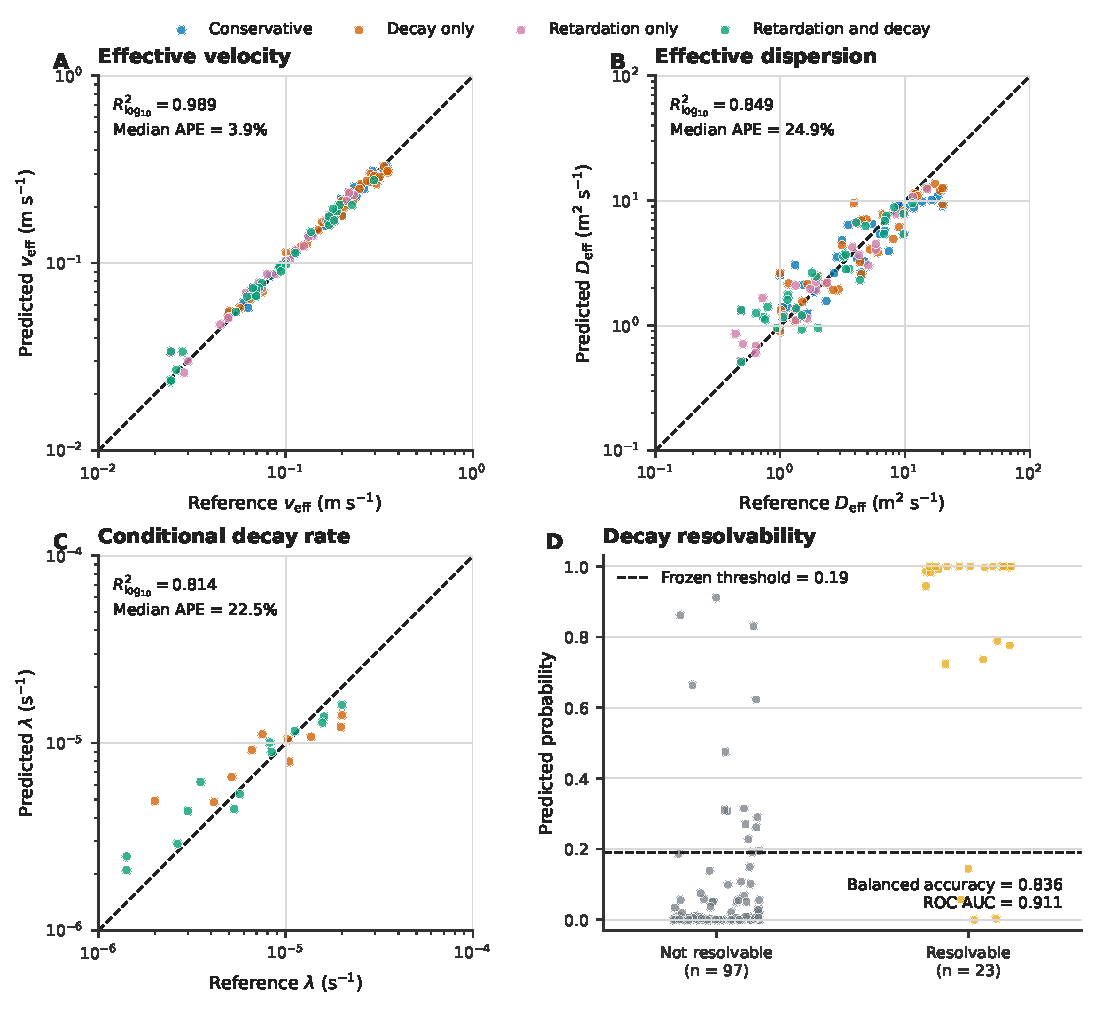
\includegraphics[width=0.91\textwidth]{figures/figure_01_parameter_model_validation.pdf}
\caption{Validación de ADR1D-ML sobre 120 escenarios nuevos. (A--C) Acuerdo
entre referencia y predicción agregada; la línea discontinua indica identidad.
(D) Probabilidad de resolubilidad del decaimiento y umbral congelado. Cada
punto representa un escenario base, no una realización individual de ruido.}
\label{fig:ml}
\end{figure}

\begin{table}[htbp]
\centering
\caption{Criterios principales de ADR1D-ML sobre el desafío bloqueado.}
\label{tab:mlcriteria}
\small
\begin{tabularx}{\textwidth}{@{}YrrC@{}}
\toprule
Métrica & Observado & Criterio & Evaluación \\
\midrule
Mediana APE de $v_{\mathrm{eff}}$ & 3.95\,\% & $\leq10$\,\% & \pass \\
Percentil 90 APE de $v_{\mathrm{eff}}$ & 10.87\,\% & $\leq25$\,\% & \pass \\
$R^2_{\log_{10}}$ de $v_{\mathrm{eff}}$ & 0.9892 & $\geq0.90$ & \pass \\
Mediana APE de $D_{\mathrm{eff}}$ & 24.94\,\% & $\leq40$\,\% & \pass \\
Percentil 90 APE de $D_{\mathrm{eff}}$ & 65.81\,\% & $\leq100$\,\% & \pass \\
$R^2_{\log_{10}}$ de $D_{\mathrm{eff}}$ & 0.8494 & $\geq0.50$ & \pass \\
Exactitud balanceada de resolubilidad & 0.8357 & $\geq0.65$ & \pass \\
Área ROC de resolubilidad & 0.9113 & $\geq0.70$ & \pass \\
Mediana APE de $\lambda$ condicional & 22.51\,\% & $\leq85$\,\% & \pass \\
$R^2_{\log_{10}}$ de $\lambda$ condicional & 0.8139 & $\geq0.10$ & \pass \\
\bottomrule
\end{tabularx}
\end{table}

La clasificación produjo 82 verdaderos negativos, 15 falsos positivos, cuatro
falsos negativos y 19 verdaderos positivos. La sensibilidad fue 0.8261, pero
la precisión fue 0.5588. La especificidad fue 0.8454 y su promedio con la
sensibilidad produce la exactitud balanceada de 0.8357. En otras palabras, el
modelo recuperó 19 de los 23 casos resolubles, pero solo 19 de sus 34
declaraciones positivas fueron correctas. Este comportamiento puede ser
razonable para una etapa de cribado si un falso negativo es más costoso, pero
esa preferencia no fue parte del protocolo y no debe suponerse para una decisión
concreta. Una clase positiva señala que conviene examinar el decaimiento; no lo
confirma por sí sola.

La regresión condicional se evaluó en 23 escenarios, por encima del mínimo de
diez fijado para aplicar el criterio. El intervalo bootstrap del 95\,\% para su
mediana APE fue 16.59--38.93\,\%. Los intervalos correspondientes fueron
0.0255--0.0395 para el RMSE logarítmico de velocidad, 0.1524--0.1962 para el
RMSE logarítmico de dispersión, 0.7418--0.9115 para exactitud balanceada y
0.8089--0.9856 para área ROC.

El ruido afectó de manera desigual las salidas. La mediana del coeficiente de
variación entre réplicas fue 0.66\,\% para velocidad, 2.82\,\% para dispersión
y 6.21\,\% para decaimiento condicional. El percentil 90 de la desviación
estándar de la probabilidad fue 0.274, aun cuando la mediana fue 0.007. Por
tanto, la estabilidad general de la clasificación no implica igual estabilidad
probabilística cerca del umbral. Las cinco clases individuales coincidieron en
96 de los 120 escenarios; en los otros 24, al menos una réplica quedó del lado
opuesto de 0.19. Conservar las cinco probabilidades permite ver esa sensibilidad
que una única etiqueta agregada oculta.

Entre regímenes, la mediana APE de dispersión varió de 16.22\,\% en solo
retardación a 30.73\,\% en solo decaimiento; el $R^2$ logarítmico permaneció
entre 0.806 y 0.882. La velocidad fue más uniforme, con medianas APE entre
3.31\,\% y 4.07\,\%. La evidencia respalda mejor la estimación de velocidad que
una lectura intercambiable de todas las salidas. En particular, no conviene
propagar velocidad, dispersión y decaimiento hacia una simulación posterior
como si compartieran el mismo error relativo.

\subsection{Predicción de campos con ADR1D-NN}

Sobre 299,880 puntos, ADR1D-NN obtuvo MAE de 0.00629, RMSE de 0.02258 y
$R^2=0.98937$. En la región activa, el RMSE aumentó a 0.03887. La mediana del
RMSE por escenario fue 0.01923, el percentil 90 fue 0.03100 y el máximo fue
0.05323. La Tabla~\ref{tab:nncriteria} confirma el cumplimiento de los 12
criterios fijados.

Como la salida es $c=C/C_0$, el RMSE global corresponde a 2.26 puntos
porcentuales de la concentración de entrada y el RMSE activo a 3.89 puntos. De
los 299,880 puntos, 79,556 (26.5\,\%) pertenecieron a la región activa y 220,324
(73.5\,\%) a la región inactiva. Esta asimetría explica por qué se requiere una
métrica activa además del promedio global.

\begin{table}[htbp]
\centering
\caption{Criterios principales de ADR1D-NN sobre el desafío bloqueado.}
\label{tab:nncriteria}
\small
\begin{tabularx}{\textwidth}{@{}YrrC@{}}
\toprule
Métrica & Observado & Criterio & Evaluación \\
\midrule
RMSE global & 0.02258 & $\leq0.035$ & \pass \\
RMSE en región activa & 0.03887 & $\leq0.065$ & \pass \\
$R^2$ global & 0.98937 & $\geq0.97$ & \pass \\
Percentil 90 del RMSE por escenario & 0.03100 & $\leq0.05$ & \pass \\
Mediana del error relativo de masa & 1.74\,\% & $\leq10$\,\% & \pass \\
Percentil 90 del error relativo de masa & 7.82\,\% & $\leq25$\,\% & \pass \\
Mediana del error de llegada & 1800 s & $\leq1800$ s & \pass \\
Percentil 90 del error de llegada & 1800 s & $\leq3600$ s & \pass \\
Predicciones negativas & 0 & $=0$ & \pass \\
Predicciones mayores que uno & 0 & $=0$ & \pass \\
Error máximo de condición inicial & 0 & $\leq10^{-12}$ & \pass \\
Error máximo de frontera de entrada & 0 & $\leq10^{-12}$ & \pass \\
\bottomrule
\end{tabularx}
\end{table}

Los intervalos bootstrap del 95\,\% fueron 0.02081--0.02447 para RMSE global,
0.03747--0.04047 para RMSE activo y 0.02630--0.03347 para el percentil 90 del
RMSE por escenario. El error de masa mostró un comportamiento favorable en la
mayoría de los casos, mientras que el error de llegada se concentró en 1800 s,
igual al intervalo temporal de la tabla de evaluación. Este último resultado
debe leerse con la resolución disponible: no demuestra precisión subintervalo.
La mediana del error relativo de la integral espacio-temporal fue 1.74\,\%; en
el 90\,\% de los escenarios no excedió 7.82\,\%. Esto indica buen acuerdo del
contenido integrado, pero no garantiza que ese contenido esté situado en el
mismo lugar o llegue en el mismo instante.

\begin{figure}[!t]
\centering
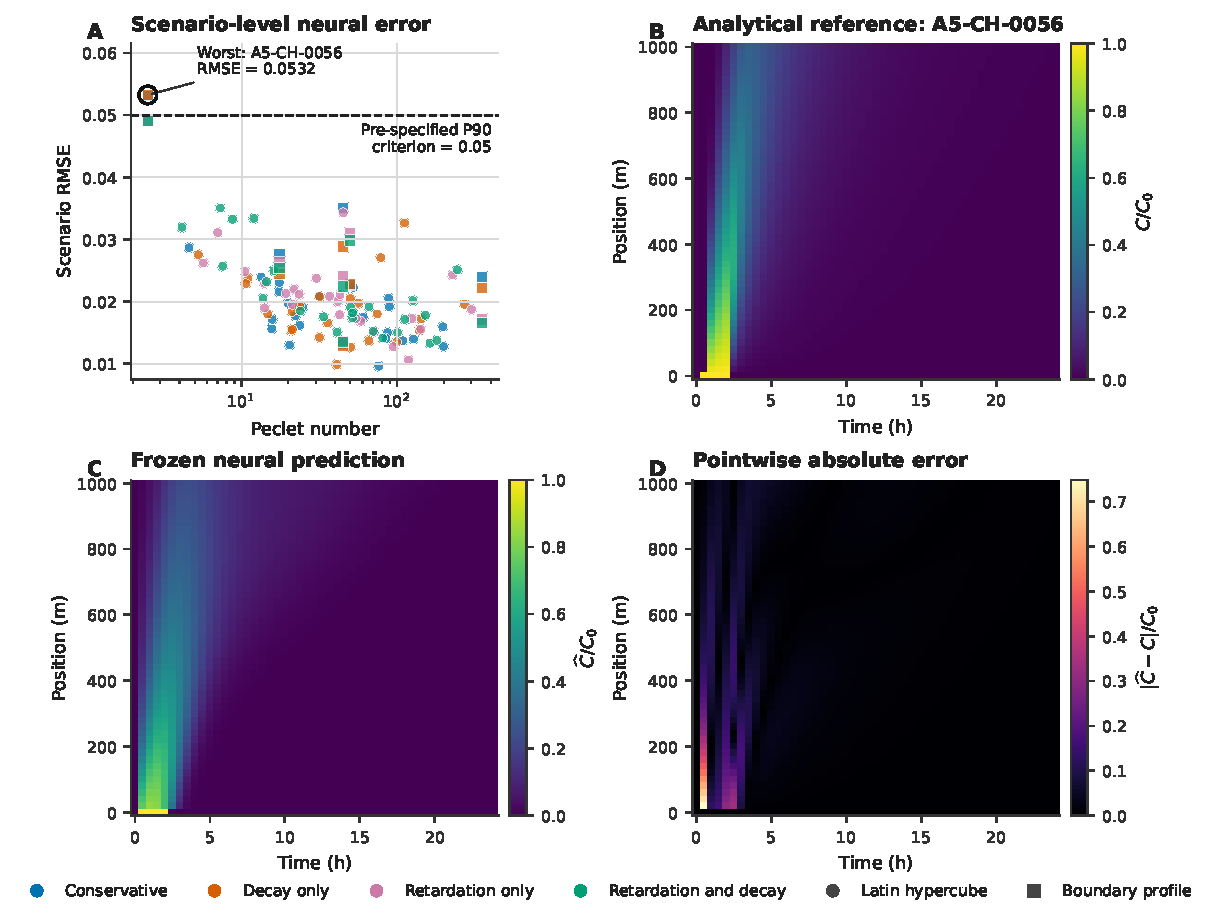
\includegraphics[width=0.92\textwidth]{figures/figure_02_neural_field_validation.pdf}
\caption{Heterogeneidad del error de ADR1D-NN. (A) RMSE por escenario frente al
número de Peclet; el criterio se aplica al percentil 90, no al máximo
individual. (B--D) Referencia analítica, predicción congelada y error absoluto
del escenario con mayor RMSE persistido, \code{A5-CH-0056}. Los cuadrados
identifican perfiles de frontera y los círculos puntos Latin hypercube.}
\label{fig:nn}
\end{figure}

El caso \code{A5-CH-0056} pertenece al régimen de solo decaimiento, fue un
perfil de frontera y tuvo $\mathrm{Pe}=2.5$. Su RMSE fue 0.05323,
$R^2=0.87276$, RMSE activo de 0.03662 y error máximo de 0.74876. La
Figura~\ref{fig:nn} muestra que la diferencia se concentra alrededor de la
evolución temprana del pulso y su frente, no de manera uniforme en las 24
horas. El máximo error puntual de todo el desafío, 0.74945, apareció en otro
perfil de frontera de Peclet 2.5, \code{A5-CH-0026}. La coexistencia de un
RMSE global bajo y errores máximos altos se explica en parte por la gran
proporción de celdas inactivas o cercanas a cero.

Los dos máximos permiten localizar el mecanismo. En \code{A5-CH-0056} y
\code{A5-CH-0026}, la fuente comienza en $t=1800$ s, la primera posición
interior es $x=20$ m y la referencia todavía vale cero en el instante exacto de
encendido. La red predijo 0.74876 y 0.74945, respectivamente. El punto no está
cubierto por las restricciones duras, porque no pertenece a $t=0$ ni a $x=0$.
Se trata de una llegada interior anticipada en una discontinuidad temporal, no
de una pequeña desviación distribuida por todo el campo. Además, como la
referencia es menor que $10^{-4}$, estos máximos pertenecen por definición a la
región inactiva y no aparecen en el máximo activo.

Los perfiles de frontera tuvieron RMSE agrupado de 0.02995, frente a 0.02032 en
los puntos Latin hypercube. El cuartil inferior de Peclet mostró RMSE agrupado
de 0.03033, el mayor entre cuartiles. Sin embargo, el RMSE activo fue mayor en
el cuartil superior de Peclet (0.05117), donde el frente ocupa menos puntos y
los errores activos pesan menos en el promedio global. Estas dos observaciones
aconsejan revisar tanto regiones activas como perfiles completos. También
muestran que ``mayor Peclet'' no implica automáticamente mayor RMSE global: en
el cuartil superior hay menos celdas activas y el promedio total queda dominado
por ceros, aunque el error dentro del frente sea mayor.

No hubo valores fuera de $[0,1]$. El residuo discreto de la EDP fue
$1.961\times10^{-4}$ s$^{-1}$. Se reporta como diagnóstico: depende de la
discretización usada para calcular derivadas y no equivale a una prueba de
conservación local o de satisfacción exacta de la ecuación. Su valor tampoco se
compara directamente con $\lambda$, porque el residuo reúne derivadas temporal,
advectiva, dispersiva y reactiva, y las diferencias centradas son especialmente
sensibles a los cambios bruscos del pulso.

\subsection{Referencia numérica y refinamiento}

La implementación analítica local se contrastó primero con 39,200 valores del
campo bloqueado; la diferencia absoluta máxima fue $6.50\times10^{-12}$. Los 16
casos seleccionados se resolvieron en tres niveles, para 48 ejecuciones. El RMSE
frente a la solución analítica disminuyó de forma monótona en todos los casos.

\begin{figure}[htbp]
\centering
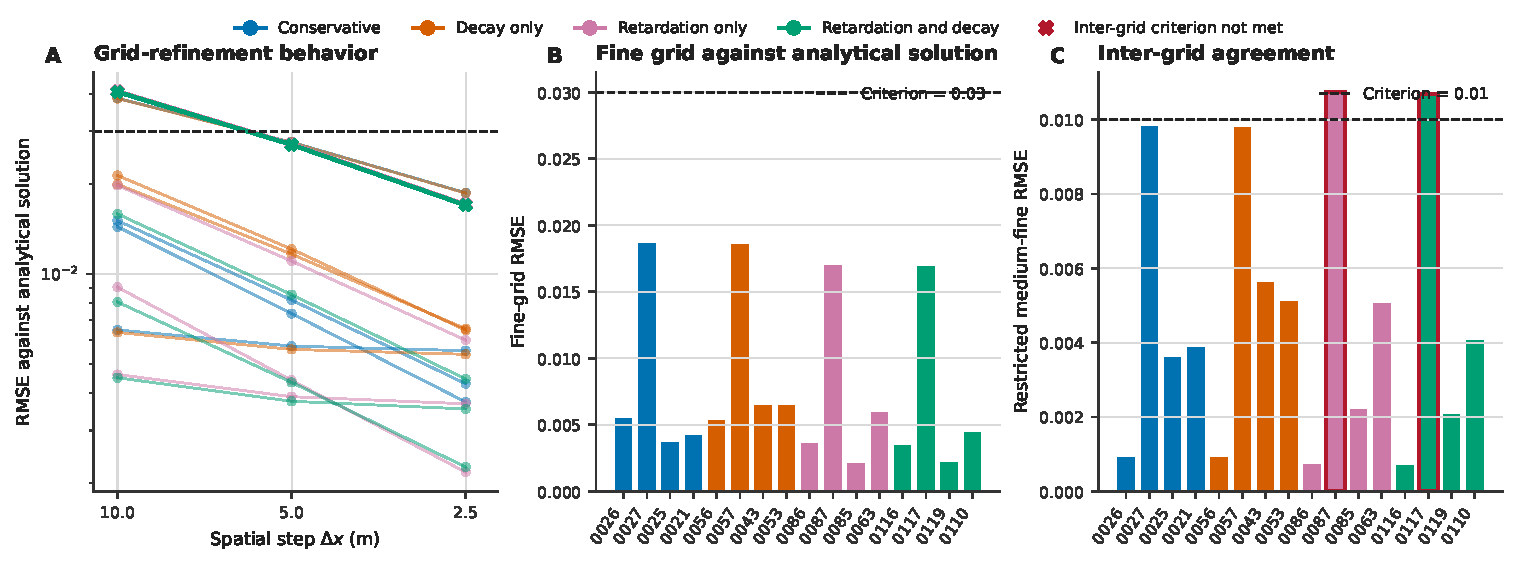
\includegraphics[width=\textwidth]{figures/figure_03_numerical_reference_convergence.pdf}
\caption{Referencia tradicional. (A) RMSE frente a la solución analítica al
refinar espacio y tiempo. (B) RMSE de la malla fina en los 16 casos. (C) RMSE
entre las mallas media y fina restringidas a puntos comunes. Los contornos
rojos marcan los dos casos que rebasaron la tolerancia entre mallas.}
\label{fig:numerical}
\end{figure}

\begin{table}[htbp]
\centering
\caption{Resumen de la referencia numérica tradicional.}
\label{tab:numerical}
\small
\begin{tabularx}{\textwidth}{@{}YrrC@{}}
\toprule
Diagnóstico & Observado & Criterio & Evaluación \\
\midrule
Mediana del RMSE fino & 0.00546 & $\leq0.03$ por caso & \pass \\
Máximo RMSE fino & 0.01867 & $\leq0.03$ por caso & \pass \\
Mediana del RMSE medio--fino & 0.00399 & $\leq0.01$ por caso & --- \\
Máximo RMSE medio--fino & 0.01074 & $\leq0.01$ por caso & \mixed \\
Mínima concentración normalizada & 0.0 & $\geq-10^{-10}$ & \pass \\
Máximo residuo absoluto de balance & $4.45\times10^{-13}$ & Diagnóstico & --- \\
\bottomrule
\end{tabularx}
\end{table}

La Tabla~\ref{tab:numerical-cases} abre el resultado agregado y permite revisar
los 16 casos sin depender de la figura. ``Medio--fino'' compara promedios de
celda en la misma malla restringida; los dos valores en negritas son los únicos
que rebasan 0.01.

\begin{table}[htbp]
\centering
\caption{Resultados individuales de la referencia tradicional. Pe y Da se
calculan con los parámetros verdaderos.}
\label{tab:numerical-cases}
\scriptsize
\setlength{\tabcolsep}{3.5pt}
\begin{tabularx}{\textwidth}{@{}p{1.9cm}Yrrrr@{}}
\toprule
Caso & Criterio de selección & Pe & Da & RMSE fino & RMSE medio--fino \\
\midrule
\multicolumn{6}{@{}l}{\textbf{Conservativo}} \\
\code{A5-CH-0026} & Pe mínimo & 2.50 & 0 & 0.00554 & 0.00094 \\
\code{A5-CH-0027} & Pe máximo & 350.00 & 0 & 0.01867 & 0.00984 \\
\code{A5-CH-0025} & Viaje advectivo máximo & 50.00 & 0 & 0.00373 & 0.00363 \\
\code{A5-CH-0021} & Medoide & 31.48 & 0 & 0.00430 & 0.00389 \\
\addlinespace
\multicolumn{6}{@{}l}{\textbf{Solo decaimiento}} \\
\code{A5-CH-0056} & Pe mínimo & 2.50 & 0.02828 & 0.00539 & 0.00094 \\
\code{A5-CH-0057} & Pe máximo & 350.00 & 0.00404 & 0.01863 & 0.00982 \\
\code{A5-CH-0043} & Da máximo & 74.42 & 0.13230 & 0.00649 & 0.00565 \\
\code{A5-CH-0053} & Medoide & 50.33 & 0.00441 & 0.00655 & 0.00514 \\
\addlinespace
\multicolumn{6}{@{}l}{\textbf{Retardación y decaimiento}} \\
\code{A5-CH-0116} & Pe mínimo & 2.50 & 0.05798 & 0.00354 & 0.00073 \\
\code{A5-CH-0117} & Pe máximo & 350.00 & 0.00828 & 0.01697 & \textbf{0.01069} \\
\code{A5-CH-0119} & Da máximo & 44.72 & 0.30000 & 0.00226 & 0.00208 \\
\code{A5-CH-0110} & Medoide & 51.73 & 0.01751 & 0.00445 & 0.00408 \\
\addlinespace
\multicolumn{6}{@{}l}{\textbf{Solo retardación}} \\
\code{A5-CH-0086} & Pe mínimo & 2.50 & 0 & 0.00368 & 0.00073 \\
\code{A5-CH-0087} & Pe máximo & 350.00 & 0 & 0.01704 & \textbf{0.01074} \\
\code{A5-CH-0085} & Viaje advectivo máximo & 50.00 & 0 & 0.00218 & 0.00223 \\
\code{A5-CH-0063} & Medoide & 58.58 & 0 & 0.00601 & 0.00509 \\
\bottomrule
\end{tabularx}
\end{table}

Catorce escenarios cumplieron todos los criterios. \code{A5-CH-0117}
(retardación con decaimiento) y \code{A5-CH-0087} (solo retardación), ambos
seleccionados por Peclet máximo y con $\mathrm{Pe}=350$, produjeron RMSE
medio--fino de 0.01069 y 0.01074. Los excesos respecto de 0.01 fueron pequeños,
pero se conservaron sin relajar el umbral. Los dos casos sí cumplieron la
tolerancia fina frente a la solución analítica, con RMSE de 0.01697 y 0.01704.

Los excesos medio--fino fueron 6.9\,\% y 7.4\,\% respecto de la tolerancia, no
órdenes de magnitud. Aun así, su coincidencia en $\mathrm{Pe}=350$ tiene una
explicación numérica concreta. El Peclet de celda es
$P_h=\mathrm{Pe}\,\Delta x/L$: vale 1.75 en la malla media y 0.875 en la fina.
Ambas soluciones permanecen estables y no negativas gracias al ajuste
exponencial, pero representan un frente estrecho con resoluciones distintas.
El criterio entre mallas detecta ese desplazamiento aunque las dos soluciones
mantengan un RMSE menor que 0.03 frente a la analítica.

El mayor RMSE fino, 0.01867, correspondió al caso conservativo
\code{A5-CH-0027}, también con $\mathrm{Pe}=350$. Este patrón es compatible con
la mayor dificultad de resolver frentes dominados por advección a una
resolución fija. El orden observado mediano fue 0.681 del nivel grueso al medio
y 0.751 del medio al fino. Estos valores describen la campaña conjunta de
$\Delta x$ y $\Delta t$; no constituyen una estimación asintótica formal del
orden del esquema.

Todas las concentraciones fueron no negativas y el máximo residuo absoluto del
balance discreto fue $4.45\times10^{-13}$; el máximo residuo relativo fue
$2.72\times10^{-9}$. La evidencia sostiene la coherencia
de la referencia en los casos examinados, pero los dos incumplimientos entre
mallas justifican el resultado agregado \emph{evidencia mixta} y recomiendan
refinamiento adicional cuando Peclet se acerca al extremo superior del dominio.

\subsection{Costo computacional}

La Figura~\ref{fig:cost} y la Tabla~\ref{tab:cost} presentan las medianas de
siete repeticiones. Los intervalos intercuartílicos fueron estrechos respecto
de las medianas y cada carga produjo una salida idéntica en los dos
calentamientos, las siete repeticiones medidas y la sonda separada de memoria.

\begin{figure}[htbp]
\centering
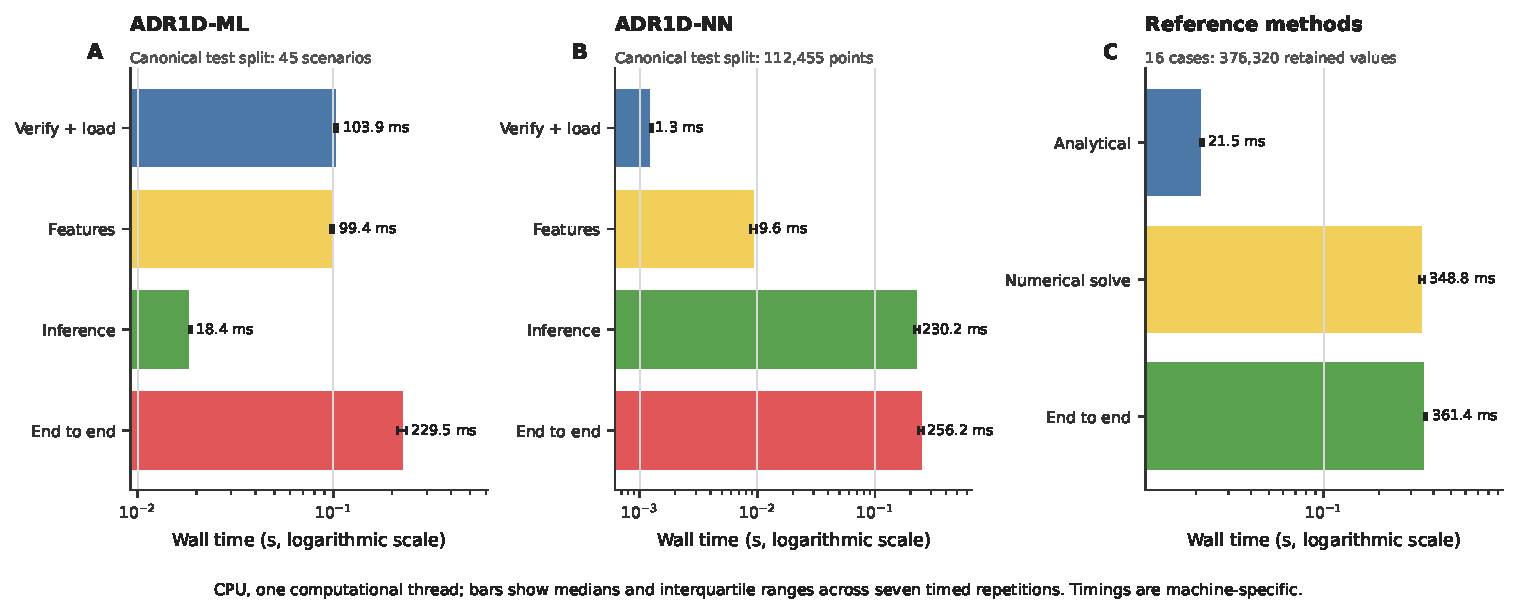
\includegraphics[width=\textwidth]{figures/figure_04_computational_cost.pdf}
\caption{Costo computacional por componente. Las barras indican mediana y rango
intercuartílico. Cada panel tiene una carga diferente y no debe usarse para
calcular una aceleración directa entre modelos o métodos.}
\label{fig:cost}
\end{figure}

\begin{table}[htbp]
\centering
\caption{Tiempos de pared en CPU con un hilo. IQR: rango intercuartílico.}
\label{tab:cost}
\small
\begin{tabularx}{\textwidth}{@{}Yrrr@{}}
\toprule
Carga & Mediana (ms) & IQR (ms) & Rendimiento mediano \\
\midrule
ADR1D-ML: verificar y cargar paquete & 103.87 & 2.90 & 9.63 cargas s$^{-1}$ \\
ADR1D-ML: construir 45 filas & 99.41 & 3.02 & 452.7 escenarios s$^{-1}$ \\
ADR1D-ML: inferir 45 escenarios & 18.44 & 0.42 & 2441.0 escenarios s$^{-1}$ \\
ADR1D-ML: extremo a extremo & 229.54 & 23.17 & 196.0 escenarios s$^{-1}$ \\
\addlinespace
ADR1D-NN: verificar y cargar red & 1.25 & 0.04 & 799.5 cargas s$^{-1}$ \\
ADR1D-NN: construir 112,455 filas & 9.55 & 1.11 & $1.177\times10^7$ puntos s$^{-1}$ \\
ADR1D-NN: inferir 112,455 puntos & 230.24 & 23.24 & $4.884\times10^5$ puntos s$^{-1}$ \\
ADR1D-NN: extremo a extremo & 256.23 & 20.80 & $4.389\times10^5$ puntos s$^{-1}$ \\
\addlinespace
Referencia analítica: 376,320 valores & 21.50 & 0.75 & $1.750\times10^7$ valores s$^{-1}$ \\
Solución tradicional: 376,320 valores & 348.84 & 20.20 & $1.079\times10^6$ valores s$^{-1}$ \\
Referencia numérica extremo a extremo & 361.36 & 9.27 & $1.041\times10^6$ pares s$^{-1}$ \\
\bottomrule
\end{tabularx}
\end{table}

La inferencia pura de ADR1D-ML ocupó una fracción menor del tiempo total; la
construcción de características y la verificación/carga tuvieron mayor peso.
En ADR1D-NN ocurrió lo contrario: para 112,455 puntos, la inferencia dominó el
tiempo y la construcción de entradas fue breve. En la referencia tradicional,
la solución numérica dominó sobre la evaluación analítica.

Cada fila representa un lote completo, no el costo fijo de una predicción
aislada. El rendimiento en escenarios o puntos por segundo resulta de dividir
la cardinalidad del lote entre su tiempo mediano y puede cambiar con otro tamaño
de lote. En un servicio que mantiene el modelo en memoria, el costo de carga se
amortizaría; en una ejecución de línea de comandos que se inicia para cada
consulta, volvería a pagarse. Este estudio informa ambos componentes, pero no
simula un servicio persistente.

Estas cifras describen un equipo Apple arm64 con macOS 26.5.2, 10 CPU lógicas,
24 GiB de memoria y CPython 3.12.2. Se usaron NumPy 2.0.2, pandas 2.2.3,
SciPy 1.15.2, scikit-learn 1.7.0, joblib 1.4.2 y PyTorch 2.7.1. Las cargas no son
equivalentes: ADR1D-ML resuelve un problema inverso por escenario, ADR1D-NN
evalúa un sustituto puntual y la referencia numérica conserva valores de 16
casos en una malla distinta. Por ello no se calcula un factor de aceleración.

La solución analítica fue la operación más rápida de las cargas de campo
medidas. Esto importa para interpretar la utilidad del sustituto: en el problema
homogéneo de ADR1D, donde existe una expresión cerrada, la red no ofrece una
ventaja computacional demostrada frente a esa expresión. Su interés de
integración debe evaluarse en problemas donde la solución cerrada deje de estar
disponible o donde forme parte de un flujo más amplio. La campaña actual no
mide todavía ese escenario.

El pico trazado desde Python fue aproximadamente 27.6 MiB para carga y flujo
completo de ADR1D-ML, 25.9 MiB para el flujo completo de ADR1D-NN y 11.5 MiB
para la referencia numérica completa. Estas cantidades excluyen memoria que
las bibliotecas nativas no exponen a \code{tracemalloc}.

\section{Discusión}

\subsection{Qué demuestra la evaluación}

La principal fortaleza de la evidencia no es un único valor de $R^2$, sino la
secuencia de controles: modelos congelados, protocolo previo, desafío sin
colisiones, una sola inferencia persistida, auditoría desde salidas planas,
comparación por escenario y una referencia tradicional independiente. Dentro
de ese marco, ADR1D-ML conserva capacidad para recuperar parámetros efectivos
y ADR1D-NN reproduce campos con error agregado bajo.

Para ADR1D-ML, la velocidad es la salida más estable y precisa. La dispersión y
el decaimiento contienen más variación relativa, lo cual concuerda con la
dificultad de separar ensanchamiento, atenuación y censura a partir de seis
curvas ruidosas. La clasificación de resolubilidad tiene buena discriminación,
pero la precisión de 0.5588 impide tratar una clase positiva como confirmación
de decaimiento. Su uso más razonable es señalar escenarios que requieren una
estimación posterior o información adicional.

Para ADR1D-NN, la ausencia de valores no físicos y el cumplimiento exacto de
condiciones impuestas son propiedades útiles para integrarlo en un flujo
numérico. Aun así, las restricciones duras cubren solo partes específicas del
problema. El máximo error puntual y los perfiles de frontera muestran que una
red puede satisfacer el contrato y conservar un RMSE global favorable mientras
desplaza localmente un frente. Una validación destinada a máximos, tiempos de
llegada o umbrales de concentración debe conservar diagnósticos locales.

La campaña tradicional respalda la referencia analítica en los 16 casos y
confirma que el error disminuye al refinar. Los dos excesos entre mallas se
concentran en Peclet máximo. No invalidan las demás comparaciones, pero sí
marcan una condición concreta en la que la resolución media no puede tomarse
como equivalente a la fina bajo la tolerancia adoptada.

\subsection{Lectura conjunta de los modelos}

Aunque ADR1D-ML y ADR1D-NN pueden ocupar etapas consecutivas de un flujo de
trabajo, esta campaña los validó por separado. ADR1D-ML recibió sensores y se
comparó con parámetros verdaderos. ADR1D-NN recibió directamente los parámetros
verdaderos del desafío, no las estimaciones de ADR1D-ML. Por tanto, el RMSE de
la red cuantifica su error como sustituto cuando sus entradas físicas son
conocidas; no incluye el error de un problema inverso previo.

Esta distinción tiene consecuencias. Si una dispersión estimada con error de
25\,\% se entrega a la red, el campo resultante puede diferir de la solución
calculada con la dispersión verdadera aun cuando ADR1D-NN aproxime perfectamente
la entrada recibida. Del mismo modo, un falso positivo de resolubilidad puede
introducir un $\lambda$ positivo en un caso cuya atenuación no puede separarse
del ruido. Los errores de ambas etapas no tienen por qué sumarse linealmente y
pueden cambiar tiempos de llegada, amplitudes y áreas de maneras distintas.

En consecuencia, la evidencia actual permite integrar las interfaces en
experimentos controlados, pero no permite asignar al flujo encadenado las
métricas individuales de cualquiera de los modelos. Una validación de extremo
a extremo tendría que tomar las cinco realizaciones de sensores, propagar la
distribución de parámetros estimados por ADR1D-ML a ADR1D-NN y comparar los
campos resultantes con la referencia, sin sustituir las entradas por sus valores
verdaderos.

\subsection{Qué no demuestra}

Los escenarios nuevos pertenecen a la misma ecuación, geometría y familia de
fuentes que el benchmark de desarrollo. Son una muestra independiente dentro
del dominio, no una prueba de física distinta. La validación tampoco aporta
datos de campo con velocidad hidráulica, dispersión, porosidad y condiciones de
frontera simultáneamente observadas. Los registros WQP disponibles ofrecen
contexto de concentraciones, unidades, censura y procedencia, pero no permiten
reconstruir por sí solos un caso identificable de la Ecuación~\eqref{eq:adr}.

Los intervalos bootstrap cuantifican variación entre escenarios del diseño, no
incertidumbre predictiva para un caso individual. ADR1D-NN es determinista y no
se evaluaron ensambles, calibración probabilística ni propagación de
incertidumbre paramétrica. Tampoco se ensayó extrapolación espacial, temporal o
paramétrica.

La comparación de tiempos no separa todas las decisiones de implementación ni
representa otro hardware. En particular, cargar un bundle de árboles y cargar
un checkpoint neuronal no tienen el mismo contrato. Los rendimientos por
segundo son útiles para dimensionar esta ejecución, pero no deben generalizarse
sin repetir el benchmark en el entorno objetivo.

La Tabla~\ref{tab:claim-boundaries} resume las fronteras de interpretación.

\begin{table}[H]
\centering
\caption{Afirmaciones respaldadas y no respaldadas por la campaña.}
\label{tab:claim-boundaries}
\small
\begin{tabularx}{\textwidth}{@{}Yp{2.3cm}Y@{}}
\toprule
Pregunta & Respuesta & Razón \\
\midrule
¿Se reproducen las evaluaciones canónicas? & Sí & Los reportes reconstruidos
fueron idénticos byte por byte. \\
¿Funcionan los modelos por separado en casos nuevos dentro de ADR1D? & Sí, con
límites & Cumplieron los criterios agregados, pero conservaron falsos positivos
y errores locales grandes. \\
¿Está validado el encadenamiento ADR1D-ML $\rightarrow$ ADR1D-NN? & No & La red
recibió parámetros verdaderos, no parámetros inferidos. \\
¿Está validado el uso con datos de campo? & No & Faltan parámetros hidráulicos,
condiciones de frontera y una referencia observacional identificable. \\
¿Está demostrada la extrapolación? & No & Todos los casos pertenecen a los
rangos, la geometría y la ecuación de ADR1D. \\
¿Existe una aceleración universal? & No & Las cargas, cardinalidades y equipos
no son equivalentes; la solución analítica fue además más rápida en este caso. \\
¿Los criterios equivalen a seguridad regulatoria? & No & Son tolerancias de
ingeniería fijadas para el benchmark sintético. \\
\bottomrule
\end{tabularx}
\end{table}

\subsection{Implicaciones para integración numérica}

Los resultados apoyan una integración condicionada, no una sustitución
automática del modelo físico. Se recomienda:

\begin{enumerate}
    \item \textbf{Verificar identidad.} Comprobar el modelo, el protocolo y los
    módulos de inferencia contra sus manifiestos antes de cargar un artefacto
    evita evaluar una versión distinta de la documentada.
    \item \textbf{Validar entradas.} Rechazar o marcar posiciones, tiempos,
    parámetros y pulsos fuera de los rangos ADR1D. Una salida numéricamente
    válida no convierte una extrapolación en evidencia.
    \item \textbf{Conservar las réplicas.} En el problema inverso, mantener las
    cinco predicciones y la probabilidad de resolubilidad, no solo sus promedios
    y clases, para representar sensibilidad al ruido.
    \item \textbf{Propagar parámetros.} Si ADR1D-ML alimenta a ADR1D-NN,
    evaluar varios conjuntos plausibles de parámetros en vez de tratar una
    estimación puntual como verdad exacta.
    \item \textbf{Revisar el campo local.} Acompañar RMSE global con error en
    región activa, llegada, perfiles cerca de la fuente y máximos. Los dos
    errores cercanos a 0.75 muestran por qué este paso es necesario.
    \item \textbf{Mantener casos centinela.} Resolver con referencia analítica
    o numérica combinaciones de frontera y Peclet alto en cada versión del
    flujo integrado.
    \item \textbf{Registrar costo por componente.} Separar carga,
    transformación e inferencia en el hardware de destino antes de elegir una
    estrategia de despliegue.
    \item \textbf{Revalidar al cambiar la física.} Heterogeneidad, otras
    fronteras, una geometría multidimensional o datos de sitio constituyen un
    problema nuevo y requieren protocolo y evidencia nuevos.
\end{enumerate}

En simulaciones repetidas, ADR1D-NN puede ser útil como aproximador del campo y
ADR1D-ML como etapa inversa preliminar. Ninguno de los dos sustituye la revisión
de identificabilidad, la propagación de incertidumbre o el balance físico que
requiera la aplicación final.

\section{Amenazas a la validez y limitaciones}

\begin{itemize}
    \item \textbf{Validez externa.} El estudio es sintético, unidimensional y
    homogéneo. No cubre heterogeneidad espacial, transporte multidimensional,
    reacciones no lineales ni datos de campo completos.
    \item \textbf{Independencia física.} El desafío usa una implementación
    reconstruida de la misma solución analítica y los mismos rangos físicos.
    La independencia proviene de las muestras, el bloqueo y la auditoría, no de
    una teoría de transporte diferente.
    \item \textbf{Dependencia entre benchmark y modelos.} Tanto las etiquetas
    de desarrollo como las del desafío proceden de ADR1D. La ausencia de
    colisiones evita repetir escenarios, pero no elimina supuestos compartidos
    sobre homogeneidad, linealidad, pulso rectangular y parámetros constantes.
    \item \textbf{Referencia tradicional.} Se evaluaron 16 casos y tres mallas.
    Esta selección cubre extremos y medoides, pero no constituye un barrido
    exhaustivo de convergencia.
    \item \textbf{Resolución temporal.} Los diagnósticos de llegada usan pasos
    de 1800 s en el campo de desafío; errores iguales a ese valor están
    cuantizados por la tabla de evaluación.
    \item \textbf{Ruido.} El modelo de sensores representa una sola combinación
    de error gaussiano, piso absoluto, censura y sustitución. No cubre deriva,
    dependencia temporal, sesgo de calibración o fallas de sensores.
    \item \textbf{Decaimiento condicional.} La regresión de $\lambda$ se resume
    con 23 escenarios resolubles. Sus intervalos son más amplios que los de
    velocidad y deben conservarse al comunicar precisión.
    \item \textbf{Definición de resolubilidad.} El umbral
    $1-\exp(-\mathrm{Da})\geq0.03$ relaciona atenuación ideal y ruido relativo,
    pero no incorpora el piso absoluto, la censura ni todas las correlaciones
    entre parámetros. Es una definición operativa del benchmark, no un límite
    universal de detectabilidad experimental.
    \item \textbf{Acoplamiento no evaluado.} ADR1D-NN recibió parámetros
    verdaderos. El estudio no cuantifica cómo se propagan hacia el campo los
    errores y decisiones de ADR1D-ML.
    \item \textbf{Discontinuidades.} La fuente rectangular cambia de forma
    instantánea. Los mayores errores neuronales aparecen precisamente junto al
    encendido y la primera celda interior; otras formas de fuente podrían
    cambiar la distribución del error.
    \item \textbf{Memoria y tiempo.} El benchmark se realizó en una máquina. La
    sonda de memoria de Python puede omitir asignaciones nativas y no equivale a
    memoria residente máxima.
    \item \textbf{Criterios.} Las tolerancias fueron fijadas antes del desafío,
    pero son criterios de ingeniería para este estudio, no estándares de
    calidad de agua ni garantías para decisiones públicas.
\end{itemize}

\section{Reproducibilidad y trazabilidad}

Todos los resultados se almacenaron en formatos abiertos CSV o JSON. El
protocolo legible por máquina se encuentra en
\path{configs/validation_protocol.json}. La evidencia principal se ubica en
\path{results/}; los generadores y validadores están en \path{src/}. Solo
\path{src/evaluate_locked_challenge.py} ejecutó inferencia nueva sobre el
desafío, una vez por modelo. La generación posterior de figuras leyó
exclusivamente resultados persistidos y dejó constancia de
\code{model\_loading\_or\_inference = false}.

La reproducibilidad se organizó en tres alcances. La \emph{verificación de
integridad} confirma que cada archivo esperado existe y corresponde al registro
machine-readable. La
\emph{auditoría de resultados} vuelve a calcular métricas e intervalos desde
predicciones persistidas, sin consultar los modelos. La \emph{reconstrucción
completa} vuelve a generar casos o ejecutar modelos y debe hacerse en un
directorio temporal para no confundir una réplica con la evidencia histórica.
El manifiesto final utiliza los dos primeros alcances; no incrementa el contador
de inferencias del desafío.

Las rutas almacenadas en los manifiestos son relativas a la carpeta de la
validación, de modo que el conjunto puede moverse a otra computadora sin
reescribir rutas absolutas. Cada JSON registra versiones, semillas, conteos e
información de integridad de sus insumos. Las huellas criptográficas empleadas
por los validadores permanecen en esos archivos y no se duplican en el informe.

\begin{table}[htbp]
\centering
\caption{Registros principales de trazabilidad y contenido documentado.}
\label{tab:traceability}
\small
\begin{tabularx}{\textwidth}{@{}Yl@{}}
\toprule
Artefacto & Estado o contenido \\
\midrule
\path{validation_protocol.json} & Protocolo bloqueado \\
\path{challenge_scenarios.csv} & 120 escenarios \\
\path{challenge_analytical_field.csv} & 299,880 valores \\
\path{challenge_sensor_observations.csv} & 176,400 observaciones \\
\path{canonical_reproduction.json} & Reproducción completa \\
\path{challenge_result_validation.json} & Auditoría aprobada \\
\path{numerical_reference_cases.csv} & 48 ejecuciones \\
\path{numerical_reference_metrics.json} & Evidencia mixta \\
\path{computational_cost.json} & 11 cargas medidas \\
\path{figure_manifest.json} & Ocho archivos gráficos \\
\bottomrule
\end{tabularx}
\end{table}

Los cuatro gráficos se almacenan en PDF y PNG. Dos renderizaciones temporales
independientes produjeron archivos idénticos en los ocho formatos. El
manifiesto registra los insumos, el generador y cada figura, así como el criterio
que seleccionó \code{A5-CH-0056} para la inspección de campo.

La auditoría del costo verificó 14 artefactos antes y después, sin cambios, y
registró cero inferencias de desafío y cero predicciones nuevas persistidas.
El reporte de costo reprodujo además los resultados canónicos de ambos modelos
y los RMSE de la referencia numérica dentro de tolerancias menores que
$10^{-12}$.

El informe también forma parte de la trazabilidad. La fecha interna y el
identificador del remolque PDF se fijaron antes de compilar; dos construcciones
en carpetas separadas deben producir el mismo archivo binario. Esta condición
comprueba que el documento entregado corresponde al fuente LaTeX y a las
figuras registradas, no que los resultados científicos sean correctos por el
solo hecho de compilar.

\section{Conclusiones}

La validación permite formular siete conclusiones delimitadas:

\begin{enumerate}
    \item ADR1D-ML reprodujo sus resultados canónicos y cumplió todos los
    criterios del desafío. La estimación de velocidad fue la salida más sólida;
    dispersión y decaimiento conservaron mayor incertidumbre relativa.
    \item La clasificación de resolubilidad distinguió adecuadamente las clases
    en conjunto, pero produjo 15 falsos positivos y una precisión de 0.5588. La
    probabilidad y el contexto de uso deben acompañar cualquier clase positiva.
    \item ADR1D-NN obtuvo buen ajuste global, conservó el intervalo físico e
    impuso exactamente las condiciones duras. Los errores máximos cercanos a
    0.75 y el peor RMSE de 0.05323 muestran que el resumen global no reemplaza
    el análisis de frentes y perfiles de frontera.
    \item La solución tradicional concordó con la analítica y mejoró
    monótonamente en los 16 casos. Dos escenarios de Peclet 350 no cumplieron la
    tolerancia medio--fino; el resultado numérico agregado es, por diseño,
    evidencia mixta.
    \item Los tiempos observados muestran que ambos modelos pueden evaluarse en
    fracciones de segundo para las cargas ensayadas. Las diferencias de tarea,
    malla y cardinalidad impiden convertir esas mediciones en una aceleración
    universal.
    \item Los dos modelos se validaron por separado. ADR1D-NN recibió parámetros
    verdaderos, de modo que sus métricas no describen un flujo alimentado por
    ADR1D-ML. La propagación del error inverso hacia el campo sigue pendiente de
    una evaluación específica.
    \item Los modelos están listos para integrarse en experimentos numéricos
    controlados dentro del dominio ADR1D, con verificación de entradas,
    conservación de réplicas y controles físicos. La evidencia no autoriza
    extrapolación, validación de campo ni uso regulatorio sin una campaña
    adicional.
\end{enumerate}

El siguiente paso inmediato es evaluar el encadenamiento completo dentro del
mismo dominio: sensores con ruido, parámetros inferidos, campo neuronal y
comparación final con la referencia. Después podrá estudiarse cuánto cambia la
evidencia al introducir heterogeneidad, condiciones de frontera distintas y
datos observacionales suficientes para identificar el problema físico. Cada
ampliación debe conservar el mismo orden: protocolo previo, artefactos
congelados, métricas locales y publicación de resultados favorables y
desfavorables.

\section*{Declaraciones}
\addcontentsline{toc}{section}{Declaraciones}

\textbf{Contribuciones de autoría.} Gerardo Tinoco-Guerrero, Francisco J.
Domínguez-Mota y J. Alberto Guzmán-Torres contribuyeron en igual medida al
diseño, análisis, interpretación y revisión del trabajo.

\textbf{Conflictos de interés.} Los autores declaran que no existen conflictos
de interés.

\textbf{Financiamiento y respaldo institucional.} Este trabajo recibió
financiamiento y respaldo institucional de la Secretaría de Ciencias,
Humanidades, Tecnología e Innovación (SECIHTI) de México; la Coordinación de la
Investigación Científica de la Universidad Michoacana de San Nicolás de Hidalgo
(CIC-UMSNH); SIIIA MATH: Soluciones en Ingeniería; el International Centre for
Numerical Methods in Engineering (CIMNE); y Aula CIMNE Morelia.

\textbf{Disponibilidad de datos y código.} Los datos ADR1D originales están
disponibles en \url{https://github.com/gstinoco/ADR1D}. Los modelos se publican
en \url{https://github.com/gstinoco/ADR1D-ML} y
\url{https://github.com/gstinoco/ADR1D-NN}. La evidencia específica de esta
validación se conserva junto con este informe en archivos CSV, JSON, PDF y
Python legibles y auditables.

\clearpage
\begingroup
\footnotesize
\setlength{\parskip}{0pt}
\begin{thebibliography}{99}
\setlength{\itemsep}{2pt}
\setlength{\parsep}{0pt}

\bibitem{adr1d}
G. Tinoco-Guerrero, F. J. Domínguez-Mota y J. A. Guzmán-Torres,
\emph{ADR1D: A Reproducible One-Dimensional Contaminant-Transport Benchmark},
versión 1.0.0, Universidad Michoacana de San Nicolás de Hidalgo, 2026.
\url{https://github.com/gstinoco/ADR1D}.

\bibitem{adr1dml}
G. Tinoco-Guerrero, F. J. Domínguez-Mota y J. A. Guzmán-Torres,
\emph{ADR1D-ML: Identifiable Parameter Inference for One-Dimensional Reactive
Transport}, versión 1.0.0, Universidad Michoacana de San Nicolás de Hidalgo,
2026. \url{https://github.com/gstinoco/ADR1D-ML}.

\bibitem{adr1dnn}
G. Tinoco-Guerrero, F. J. Domínguez-Mota y J. A. Guzmán-Torres,
\emph{ADR1D-NN: A Physics-Constrained Neural Surrogate for One-Dimensional
Reactive Transport}, versión 1.0.0, Universidad Michoacana de San Nicolás de
Hidalgo, 2026. \url{https://github.com/gstinoco/ADR1D-NN}.

\bibitem{ogata1961}
A. Ogata y R. B. Banks, \emph{A Solution of the Differential Equation of
Longitudinal Dispersion in Porous Media}, U.S. Geological Survey Professional
Paper 411-A, 1961. \url{https://doi.org/10.3133/pp411A}.

\bibitem{chen2011}
J.-S. Chen y C.-W. Liu, ``Generalized analytical solution for
advection-dispersion equation in finite spatial domain with arbitrary
time-dependent inlet boundary condition,'' \emph{Hydrology and Earth System
Sciences}, vol. 15, pp. 2471--2479, 2011.
\url{https://doi.org/10.5194/hess-15-2471-2011}.

\bibitem{mckay1979}
M. D. McKay, R. J. Beckman y W. J. Conover, ``A comparison of three methods for
selecting values of input variables in the analysis of output from a computer
code,'' \emph{Technometrics}, vol. 21, no. 2, pp. 239--245, 1979.
\url{https://doi.org/10.1080/00401706.1979.10489755}.

\bibitem{scharfetter1969}
D. L. Scharfetter y H. K. Gummel, ``Large-signal analysis of a silicon Read
diode oscillator,'' \emph{IEEE Transactions on Electron Devices}, vol. 16,
no. 1, pp. 64--77, 1969.
\url{https://doi.org/10.1109/T-ED.1969.16566}.

\bibitem{efron1993}
B. Efron y R. J. Tibshirani, \emph{An Introduction to the Bootstrap}.
New York: Chapman \& Hall/CRC, 1993.

\end{thebibliography}
\endgroup

\end{document}
